\documentclass[]{article}
\usepackage{graphicx}
\usepackage{hyperref}
\usepackage{amsmath}
\usepackage{caption}
\usepackage{subcaption}
\usepackage{float}


%opening
\title{VME Data Acquisition and Plastic Scintillators}
\author{Gunther T\"urk, Jonas Lehnen}

\begin{document}

\maketitle
\begin{abstract}
In this experiment we want learn how to take data via a VME module. This is shown at the example of measuring the speed of light $c$ in a plastic scintiallator. A $^{207}Bi$ source will cause by its $\beta^-$ decay a signal measurable by two photomultiplier tubes PMT. Travelling time difference and position of the sample will lead to our value of c.

\end{abstract}

\tableofcontents

\newpage
\section{Theorie}








Problem 4 

Photons with 3 MeV energy are counted by a NaI(TI) detector. Sketch the expected spectrum and explain what you sketch and the physics process beneath it. 


Problem 6 

How many counts are needed to make the standard deviation equal to 1%? And if one obtains 8423456 counts in 300 seconds, what is the standard deviation of the count rate? 
10000
0,6\%

\subsection{Radiation}\label{radiation}
\subsubsection{Radioaktive Decay}
Starting with radioaktive decay, there are three different kinds. The $\alpha$ decay is the emission of an $He^{2+}$ particle by the atoms nucleus. This radiation is blocked easily, due to large particles interaction with its surrondings. After $10cm$ of air, the exposure is no longer a threat to humans, but having an alpha emitter inside your body can lead to cancer and other dangerous diseases. The decay chanels are shown in table  \ref{tab:zerfall}

\renewcommand{\arraystretch}{1.5}
\begin{table}[H]
\centering
\begin{tabular}{c||c}
Zerfallsart & Formel   \\ \hline
$\alpha$ & $_Z^A X \rightarrow\ _2^4\alpha + _{Z-2}^{A-4} Y$ \\ \hline
$\beta^+$ &   $_Z^A X \rightarrow\  _{Z-1}^{A}Y + e^+ + \nu_e$ \\ \hline
$\beta^-$ &   $_Z^A X \rightarrow\  _{Z+1}^{A}Y + e^- +  \bar{\nu}_e$ \\ \hline
$\gamma$ &  $_Z^A X^* \rightarrow\ _Z^A X + \gamma$  \end{tabular}
\caption{Chart of radioactive decays. It is possible that the resulting nuclei are excited after their decay. Not for the $\gamma$ decay, there the nucleus' excitation is removed by a photon. }
\label{tab:zerfall}
\end{table}
\renewcommand{\arraystretch}{1}

For every decay, including the following $\beta$ decays, the mass of the starting nucleus is larger than the combined one for of the resulting nuclei. This is due to energy conservation, because kinetic energy is produced to remove a particle from the nucleus.
The $\beta$ decay is the decay of a nuclear particle, this means neutron or proton. Depending on the emission of a electron or positron, the decay is named after their charge. Additional a lepton is emitted due to conservation of the lepton number. 

These decay variations can result in a excited state of the nucleus, which is usual represented by the nuclear spin. This additional energy is released by a photon as $\gamma$ ray just like X-rays from the nucleus' electron shell. The energy results in a reassembling the nuclear particles to a lower-energy structure. The other possibility to remove this energy is by transferring it directly to a s-orbital electron, due to their positional probability in the nucleus. This leads to its emission. 

\subsubsection{Isomer}
In nuclear physics an isomer describes nuclei with the same number of protons and neutrons but different internal energy-states. Only states differing from the ground states with a long lifetime are called isomers. The difference in internal energy comes from different nuclear spins.
\subsubsection{Isomeric transition}
Isomeric transition describes a process of spontaneously changing the energy-state of the nucleus from an excited one in a lower one or the ground-state by emitting $\gamma$ radiation. The energy of the $\gamma$ depends on the specific transition, as it does in atomic physics.
\subsubsection{Internal Conversion}
Internal conversion is a special case of radioactivity. It appears when a nucleus in an excited state decays into the ground-state without emitting a photon. Instead an electron from the shell is is emitted with a specific energy. The atom remains as an ion. The kinetic energy $E_{e^-}$ of the conversion electron is the difference between the energy from the nucleus $E_{\gamma}$ and the binding energy of the shell electron $E_b$
\begin{equation}
	E_{e^-}=E_{\gamma}-E_b
\end{equation}
$E_b$ is dependent on the shell, the electron is emitted from. The spectrum of the internal conversion will show a discrete energy spectrum instead of the contiuous one from the $\beta$-decay.

\subsubsection{Interaciton of $\gamma$-rays in matter}
There are 3 main ways $\gamma$-rays can interact with matter:
\begin{enumerate}
	\item Photoeffect \newline
	If a $\gamma$ with $E_{\gamma}$ larger than the binding energy of an $e^-$ of the target material, the electron is ejected from the atomic shell and the $\gamma$ is absorbed. The kinetic energy of the electron is:
	\begin{equation}
		E_{kin}=E_{\gamma}-E_{binding}
	\end{equation}
	\item Compton scattering \\
	As compton scattering we describe an increase in the wavelength of a photon through scattering by a charged particle, usually an electron. The scattering results in a decrease of energy (increase in wavelength) of the photon, called the Compton effect. The lost energy is transferred to the electron. This process can not be explained by the wave properties of light (like Thomson- or Rayleigh-scattering) but only if we assume an elastic collision of a photon and an electron. The change in the wavelength can be calculated by the formula:
	\begin{align}\label{comption}
		\Delta \lambda&=\lambda'-\lambda \nonumber \\ 
		\Delta \lambda&=\frac{h}{m_e c}(1-\cos \Phi)		
	\end{align}
	Comption scattering is the dominating interaction for energies between 100keV and 10MeV. Below that energy the effect on the wavelength of Compton scattering is very small and its dominated by the photoelectric effect. For low energies we can observe Thomson-scattering. This is just the limit case of Compton-scattering for low energies, where the wavelength does not change.
	

	\item Pair production \\
	For high photon energies pair production is the dominating effect of light-matter interaction. In this process a photon creates an elementary particle and it's antiparticle. In order of pair production to occur, the energy of the photon needs to be at least twice as large as the rest mass of the produced particles. For the lightest elementary particle, the electron, this are  $1.022MeV$. For pair production to occur energy and momentum need to be conserved. Thus it can only happen close to a nucleus absorbing the excess momentum. The probability of pair production increases with the energy of the photon. This can be deduced from Fermis golden rule. The density of states for a certain energy is larger for two particles than for one.
\end{enumerate}
\subsubsection{Bismuth 207 decay modes}

\begin{figure}[H]
\centering
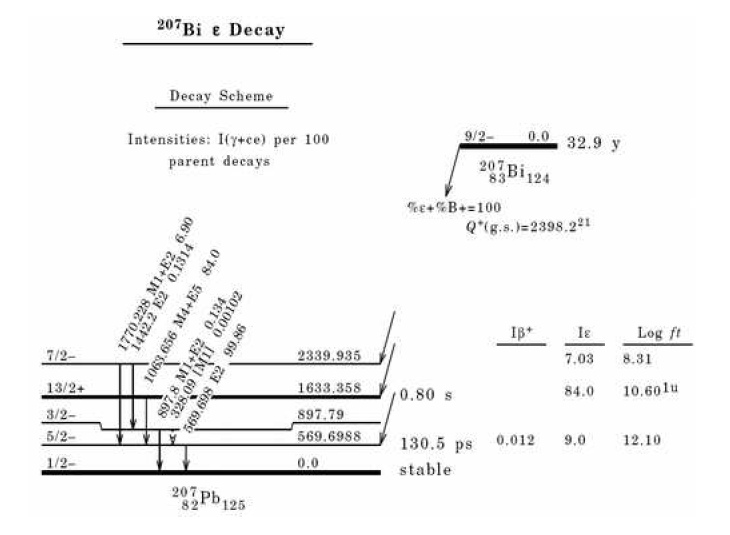
\includegraphics[width=.9\textwidth]{Plots/Bi.png}
\caption{Beta decay of bismuth Bi ends in excited nuclei of lead Pb. From there on the $\gamma$ decay happens.}
\label{fig: bi decay modes}
\end{figure}

The $\beta$ decay of the used $^{207}Bi$ source results in excited states of a $^{207}Pb$ nuclei. From there on the described $\gamma$ decay happens. In \autoref{fig: bi decay modes} the transition energies are shown. The nucleus spin is displayed with the left most numbers on a nuclei energy level. The possible transitions are shown with the arrows pointing downwards. The energy of the emitted photon is given in $keV$ and represented by the first number connected to those arrows. On the right hand side the total energy above the ground state is shown. Further right besides the energy levels the half-life time of the states is given.


\subsection{Scintillator}\label{scintillator}
A scintillator is a material that exhibits light, when excited by ionizing radiation. In our experiment we use a two meter plastic scintillator with a photomultiplier at each end to detect the decay of a Bismuth source and background radiation.

When ionizing radiation hits a scintillator it excites high energy molecule states, which then decay in multiple steps back into the ground state. Thereby they emit UV-light. This UV-light is then absorbed again by a wavelength shifter that works like the scintillator but for UV-light and that emits light in the visible spectrum. This can then be measured by the photomultiplier. Because one high energy particle can excite many high energy states until its energy is to low, the amplitude of UV light for each event is proportional to the energy of the ionizing particle.
%Haben wir photomultiplier schonmal irgendwo erklärt? das müsste sonst hier noch dran
\subsection{Photomultiplier}
If a low energy photon hits the photo cathode it ejects an electron through the photo effect. This electron is then accelerated towards several Dynodes in succession with an electric field. Every time an electron hits a dynode, it ejects several electrons from it, due to its higher energy. This leads to an exponential increase in electrons, that can then be measured as a voltage over a resistor. For this process to work the dynodes need to be on an increasingly positive potential. This is usually accomplished by a high voltage and a potential divider. 
The measured voltage is proportional to the amount of electrons hitting the photo cathode. This signal can then be used for further measurements. Depending on the shunt there is always a trade-off between precision between the amount of signals and the energy of the initial signal. 
\subsection{Refractive Index}\label{refrac index}
The refractive index is a characteristic of all materials. It determines the refractive angle if light passes different mediums according to Snell's law. 

\begin{figure}[H]
\centering
\begin{subfigure}[c]{0.48\linewidth}
\centering
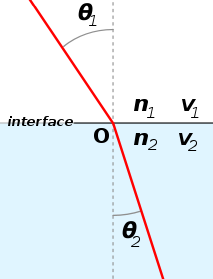
\includegraphics[width=.5\linewidth]{Plots/Snell.png}
\end{subfigure}
\begin{subfigure}{0.48\textwidth}
\begin{equation}
\frac{sin(\theta_2)}{sin(\theta_2)} =  \frac{v_2}{v_1} = \frac{n_1}{n_2} \; , \; v_i=\frac{c}{n_i}
\end{equation}
\end{subfigure}
\caption{Figure for the representation of Snell's law from en.wikipedia.org and the corresponding equation. }
\label{fig:snell}
\end{figure}

Thereby it also determines the speed of light in the medium as shown above in figure \ref{fig:snell}. On this way we will later compare our measured value with a given value for the refractive index of the plastic scintillator.


\newpage
\section{Experiment}
\subsection{Setup}\label{setup}
This experiment we are using a long and flat plastic scintillator to detect high energetic photons or charged particles like cosmic muons. The scintillator is connected with two photo multipliers (PMT) on each side, see figure \ref{fig:setup}.

\begin{figure}[H]
\centering
\begin{subfigure}[h]{0.4\textwidth}
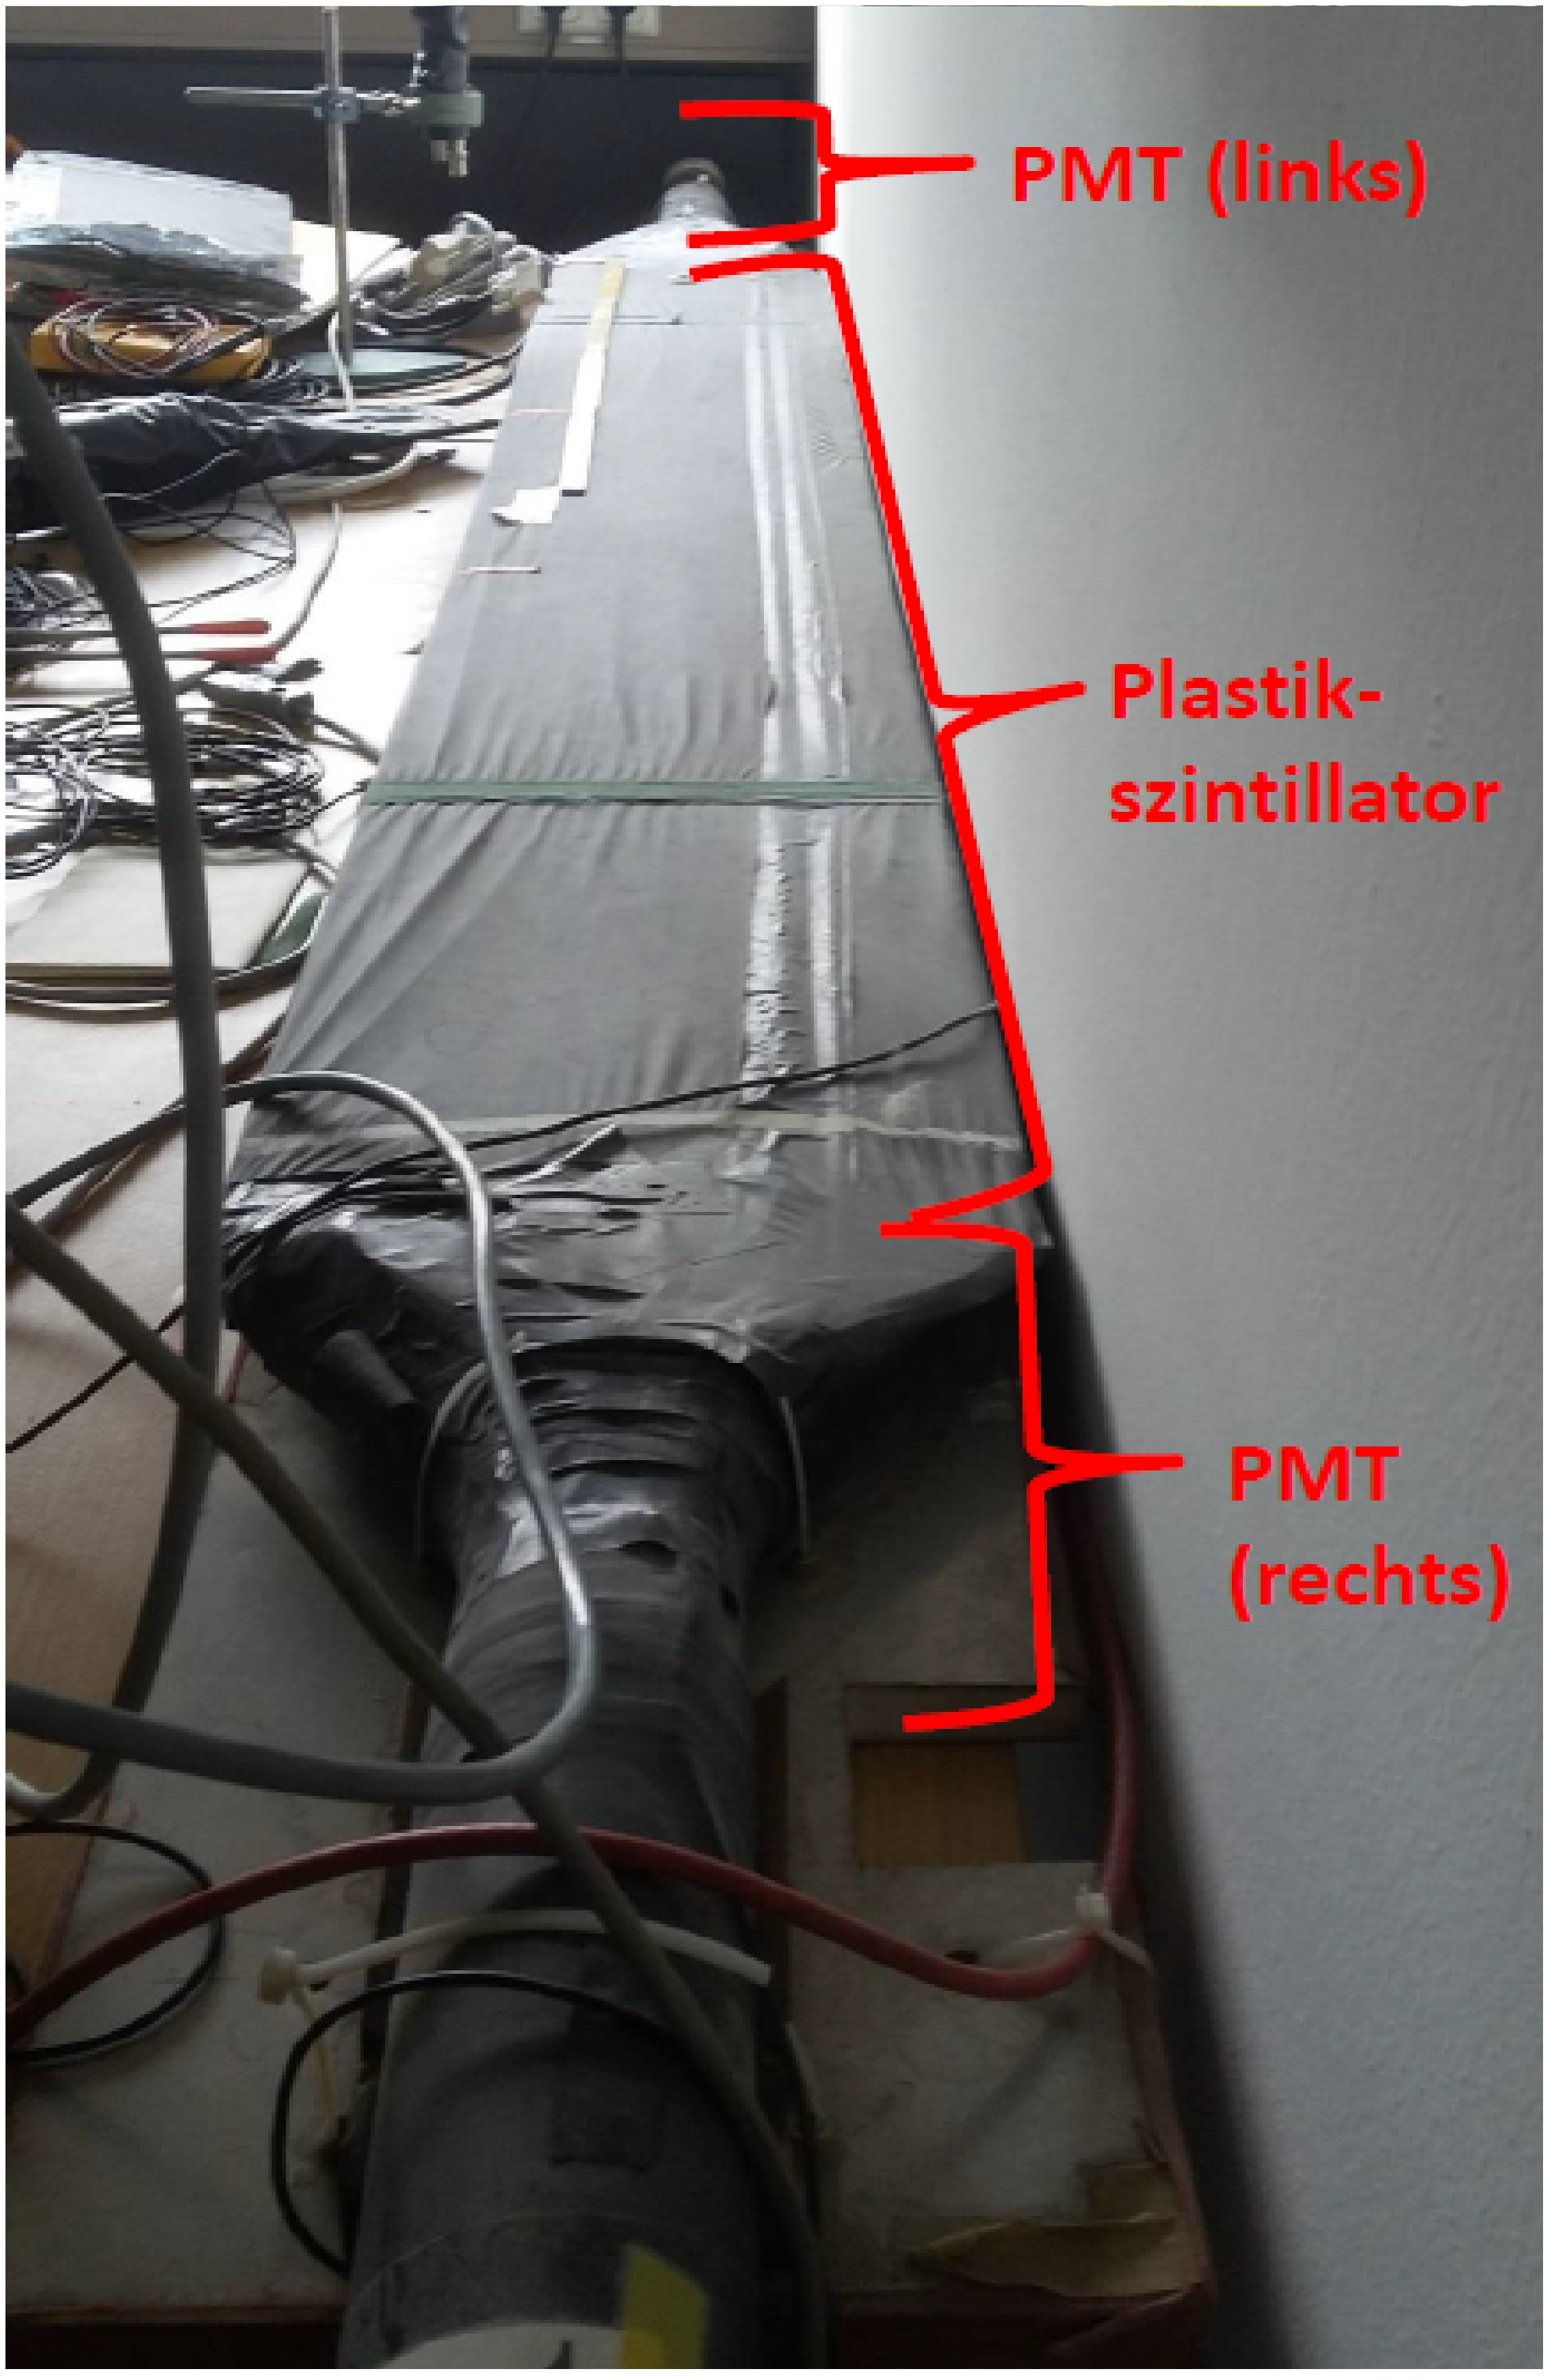
\includegraphics[width=1\textwidth]{Plots/Scintillator.jpg}
\end{subfigure}
\begin{subfigure}[h]{0.59\textwidth}
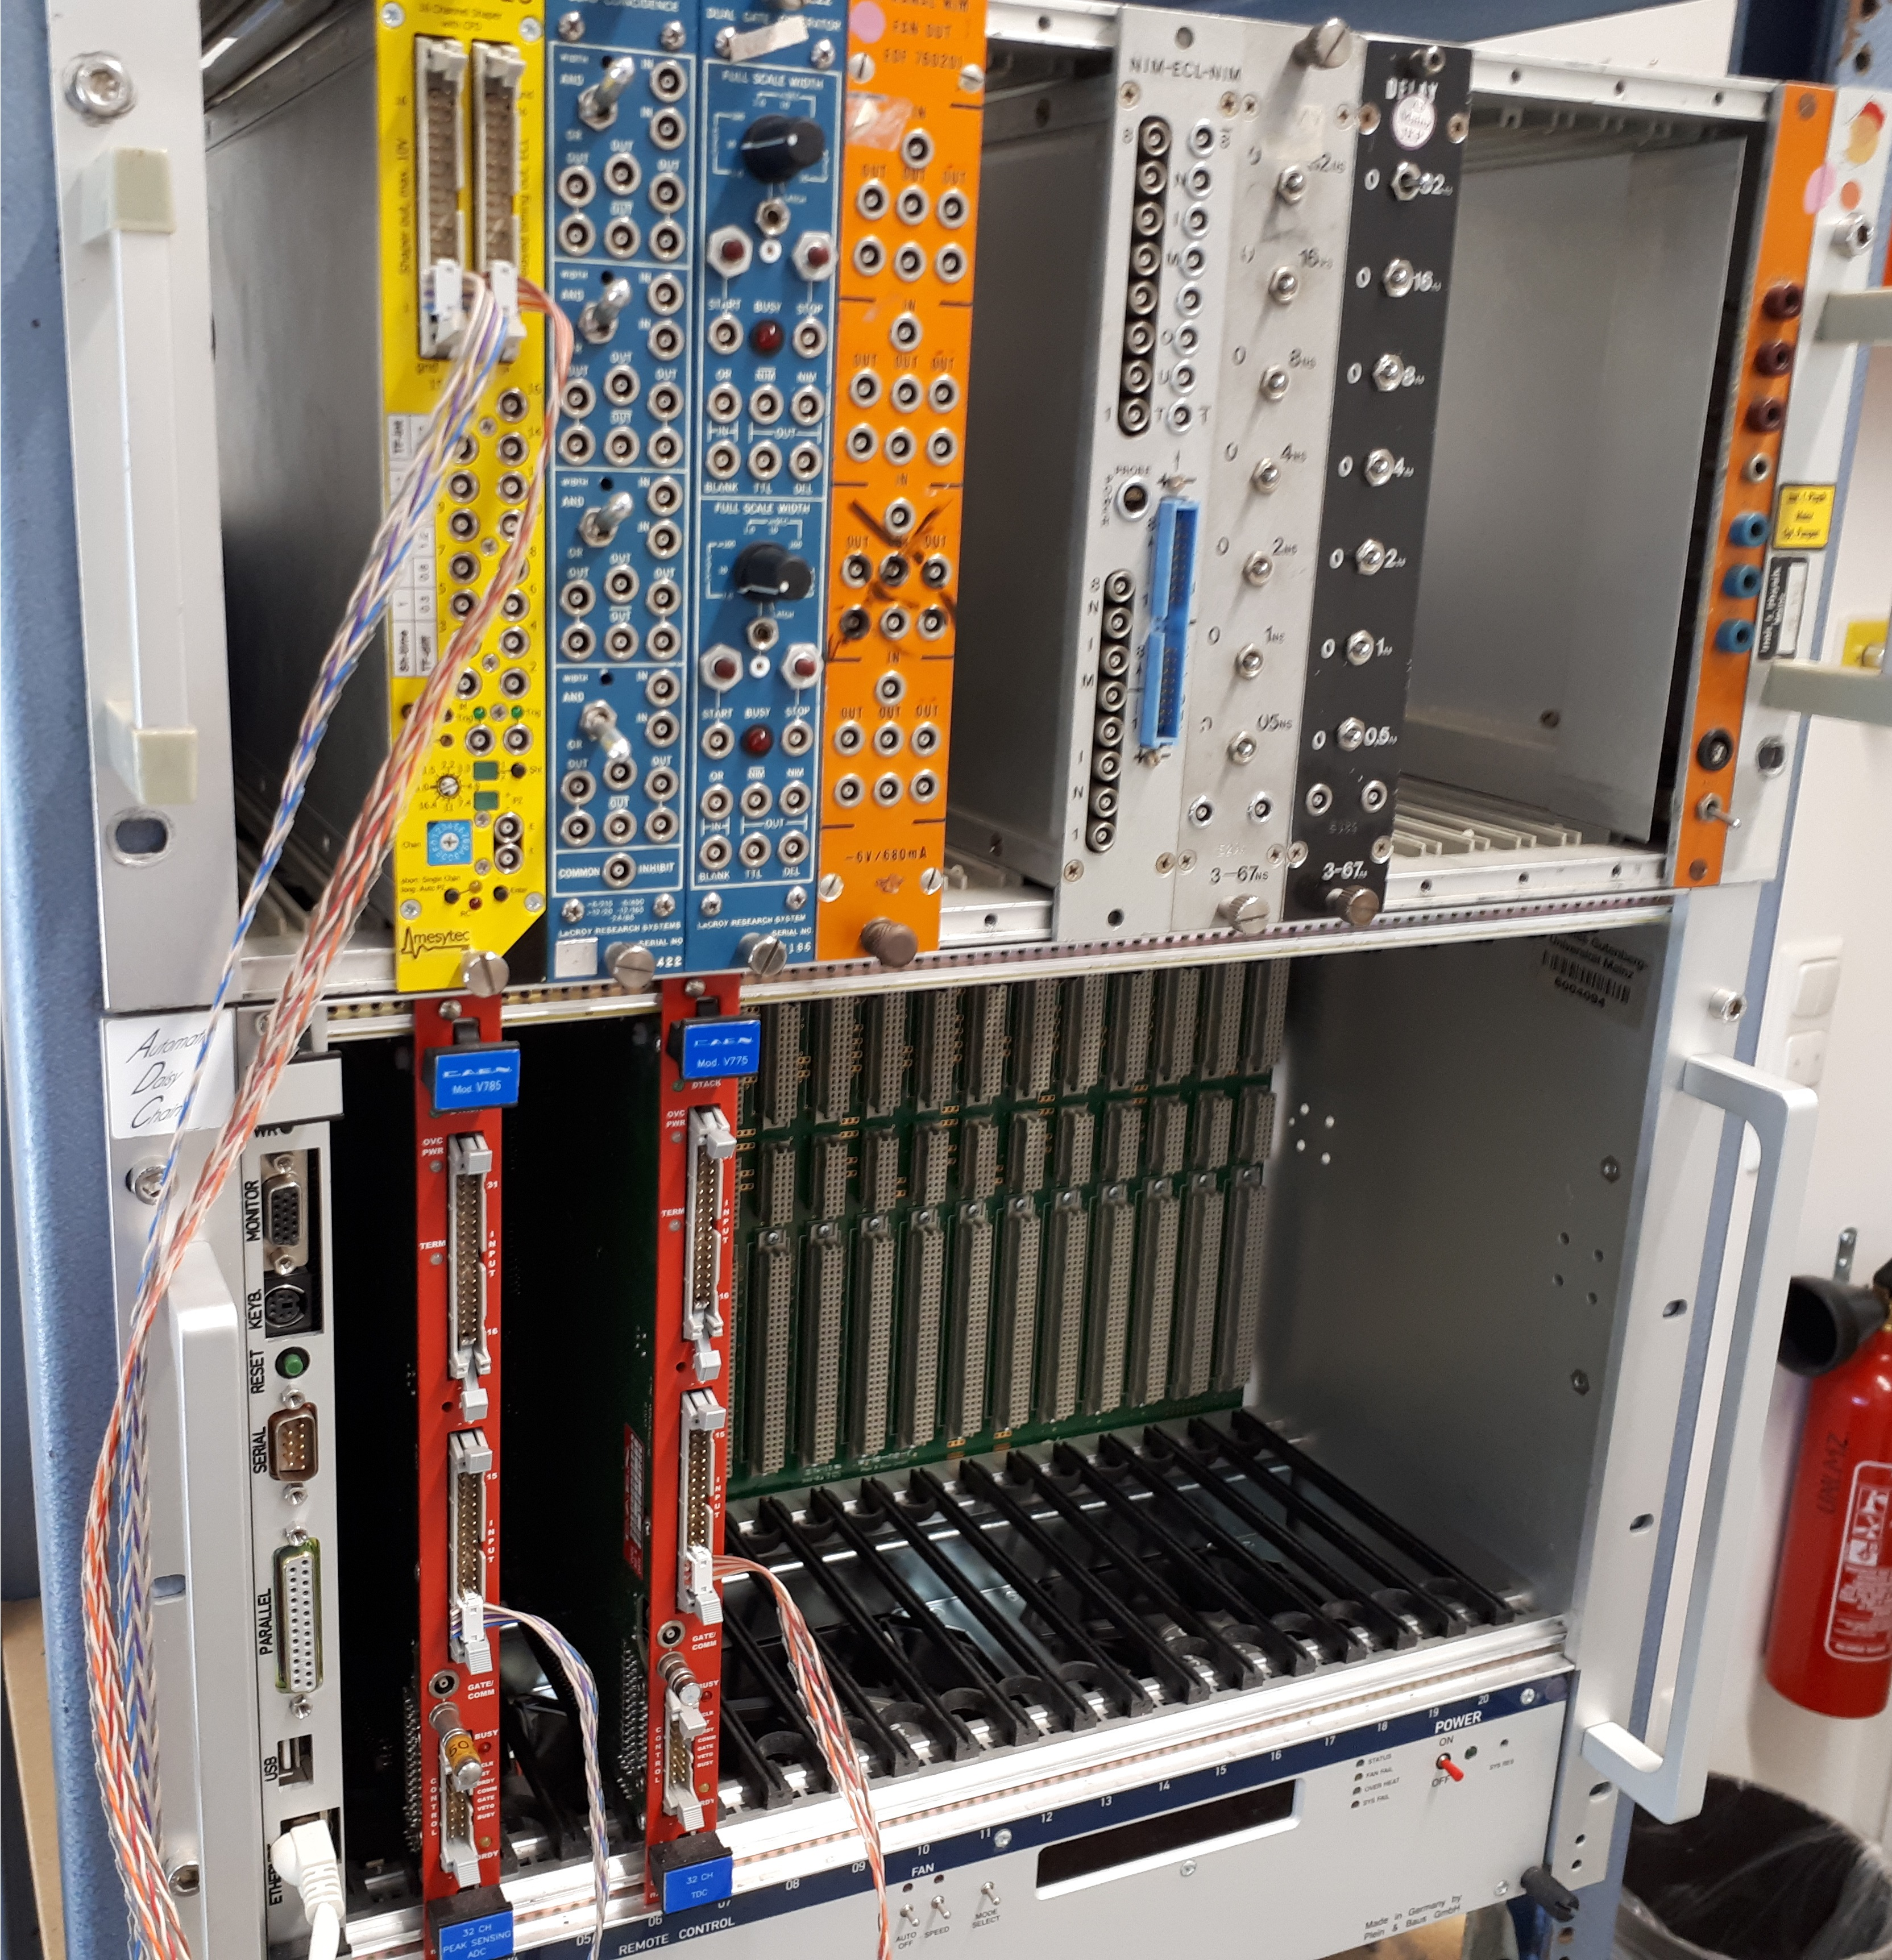
\includegraphics[width=1\textwidth]{Plots/Raw.jpg}
\end{subfigure}
\caption{Pictures of the set up. Scintillator and PMTs on the right \cite{script}. Data acquisition rack on the left without cabling. Declaration see figure \ref{fig:cabling}.}
\label{fig:setup}
\end{figure}

Both of the PMT outputs are connected with the MSCF-16 unit, the yellow one in figure \ref{fig:setup} and \ref{fig:cabling}. The L labelled cable form the left PMT and the R labelled with an additional delay from the right one. Those Delay Boxes are just more cables the signal has to pass. From the MSCF-16 on the raw data will be delayed and passed to the analogue-to-digital converter (ADC) and time-to-digital converter (TDC) on the bottom of the pictures of the rack. And there it will be processed into the data we are working with later on. Another output leads over the third black cable to the Fan-In/-Out where the signal gets copied and passed to the Dual Gate Generator.

%%%%% Platz für mehr text :D # dont float mi floats 

\begin{figure}[H]
\centering
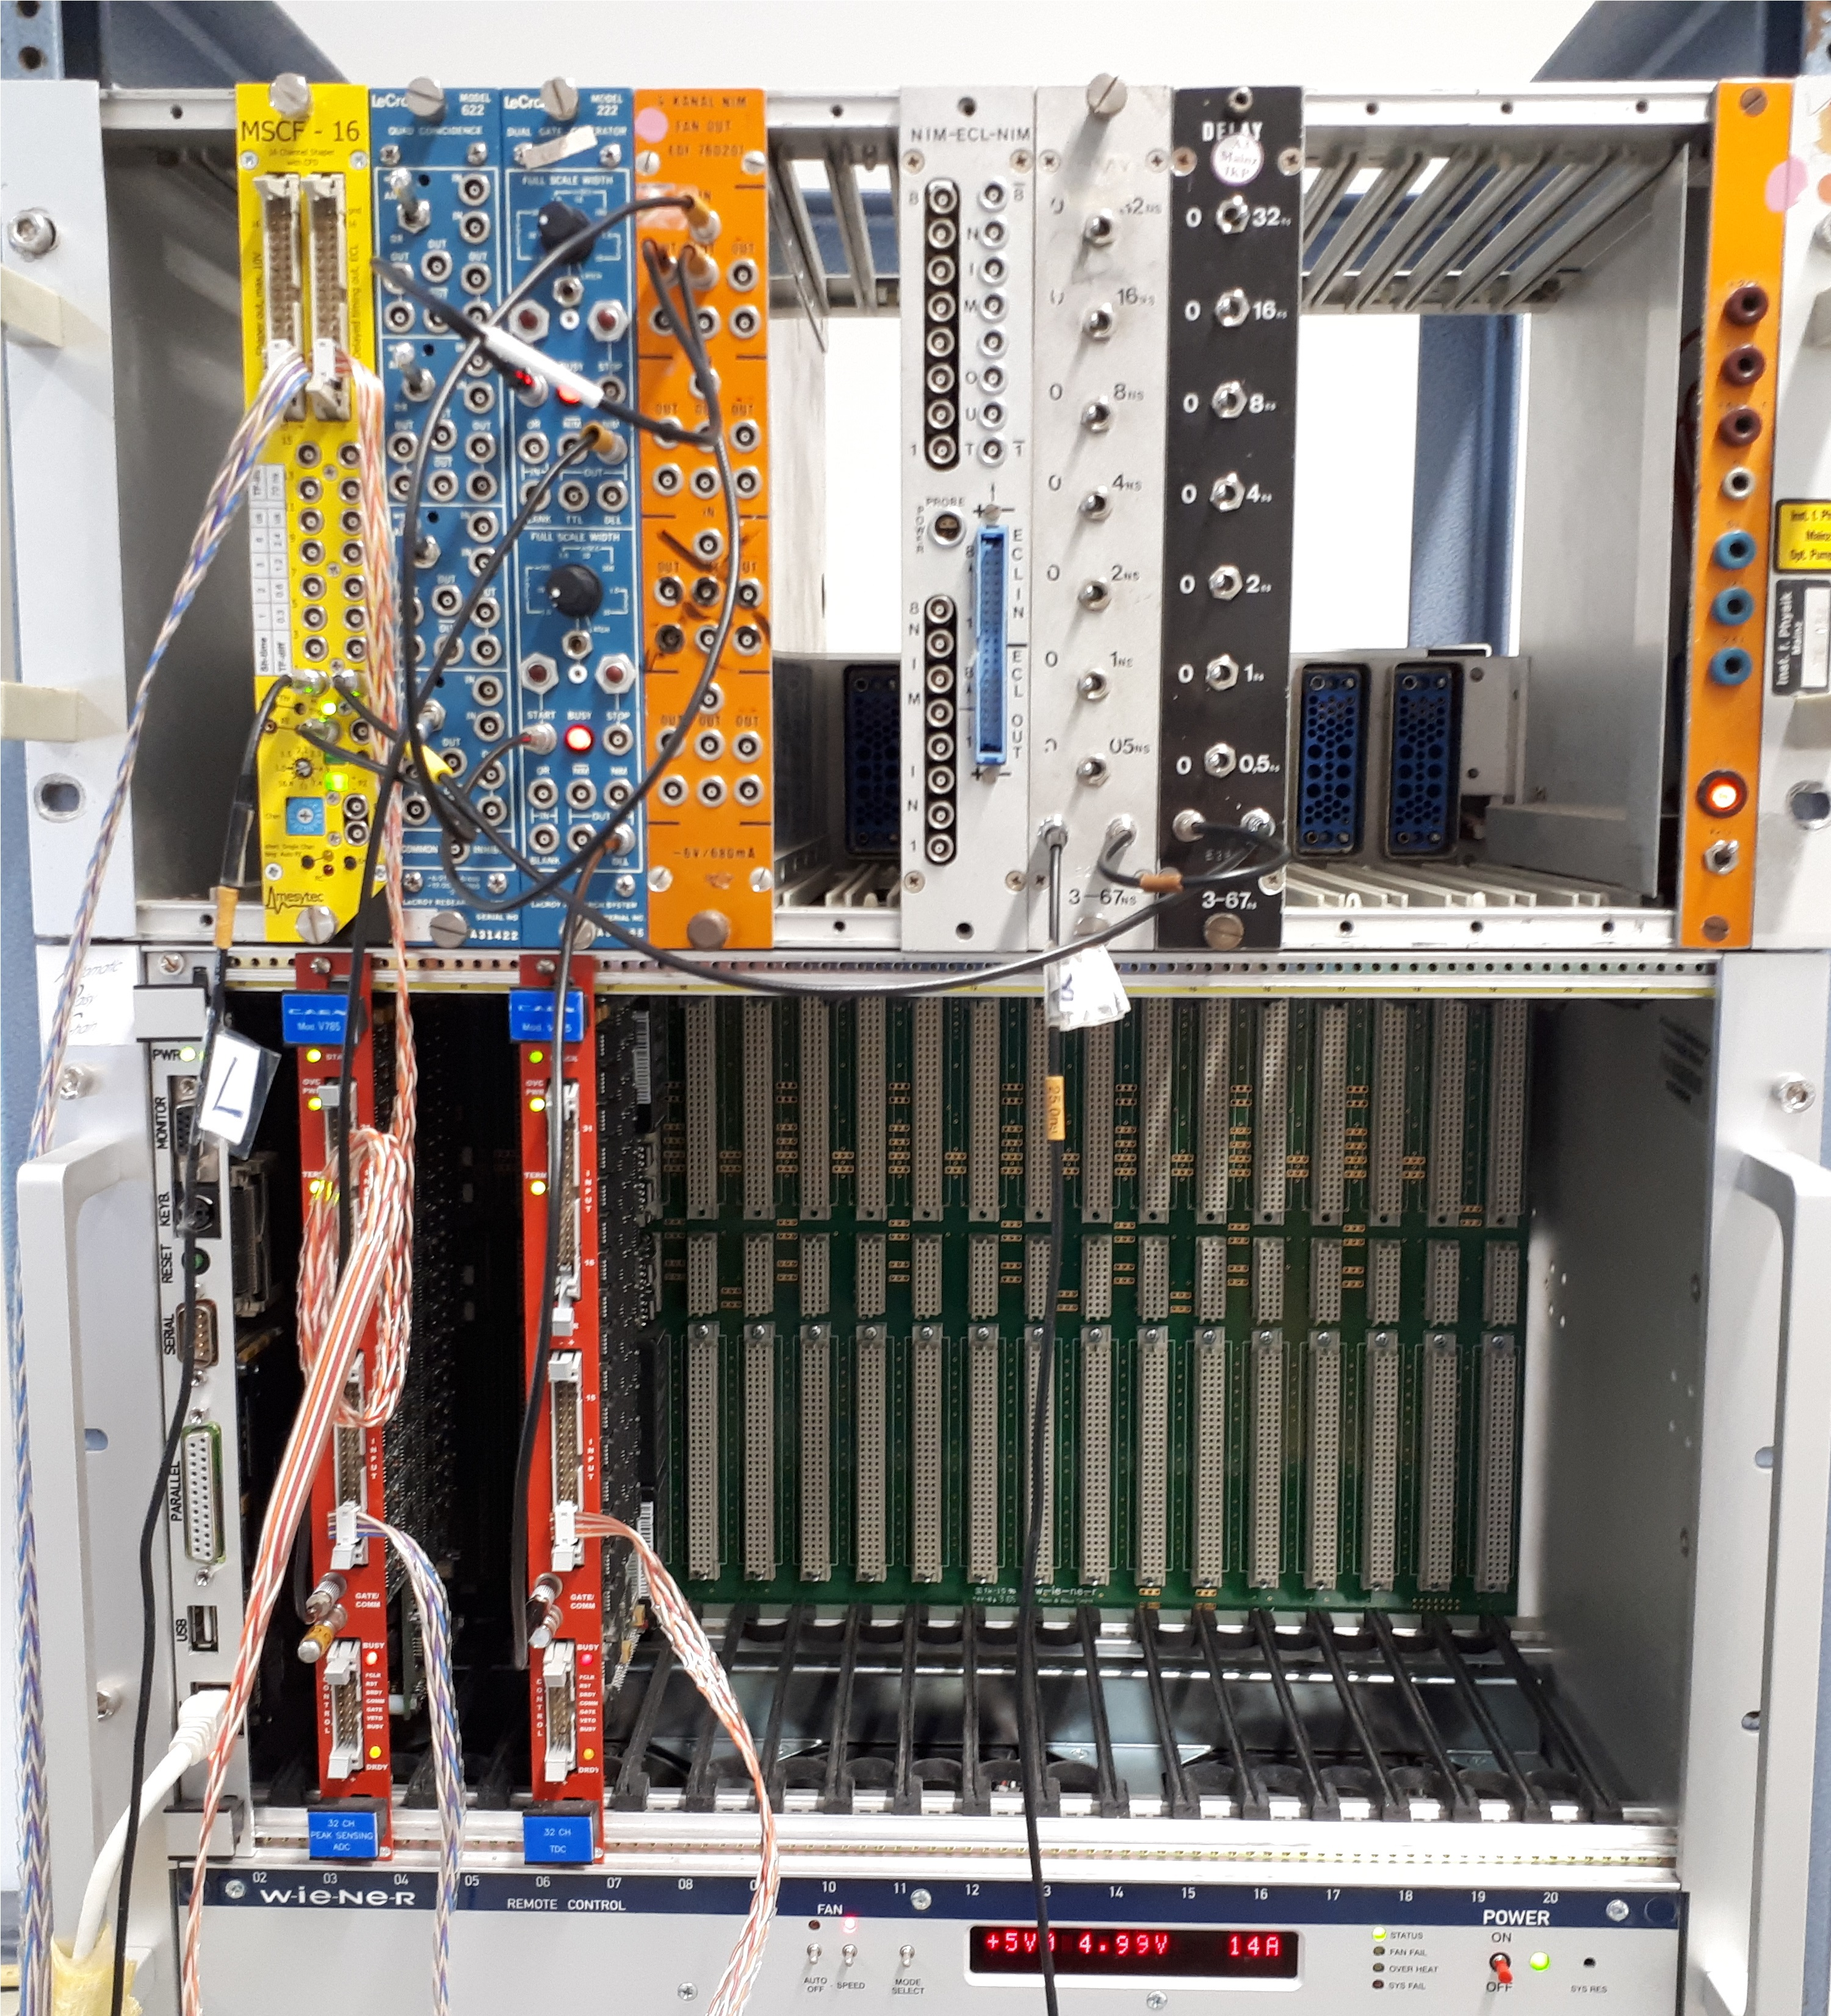
\includegraphics[width=1\textwidth]{Plots/Kabel2.jpg}
\caption{Data acquisition rack with cabling. Top left to right: MSCF-16, Quad Coincidence LeCroy 622 - not used, Dual Gate Generator LeCroy 222, Fan-In/-Out, NIM-ECL-NIM
module, two Delay Boxes.
Bottom: Gateway for PC connection, ADC, TDC.  }
\label{fig:cabling}
\end{figure}
%%%%%%%%%%%%%%%%%%%%%%%%%%%%%%%%%%%%% Kabel Schema aus Skript mit ins Bild paint'en? nää

The Gate Generators Delayed Output (DEL) produces a short signal for the TDC. This first signal starts the time measurement and gets stopped by the delayed signal of the MSCF-16. The length of the first triggering signal determines how long the second one will be measured. The ADC on the other hand receives a long signal from the gate generator. This leads to a good energy resolution but won't be necessary in this experiment.

%%% Description of how the data gets passed
\begin{figure}[H]
\centering
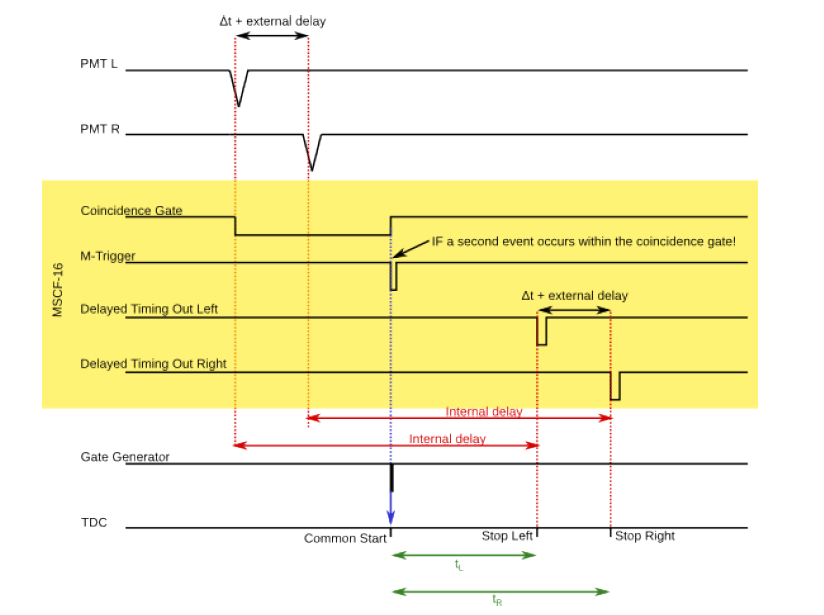
\includegraphics[width=1\textwidth]{Plots/Timing.png}
\caption{Schematic display on how the signals are passed between the components and what the TDC returns. \cite{script}}
\label{fig:timing}
\end{figure}

Now for a detailed description on what happens see figure \ref{fig:timing}. On top are the original signals the MSCF-16 receives. The signal from the right is delayed by the Delay Boxes. The first signal from the left PMT starts a coincidence gate. This is a variable time frame in which another signal has to appear to create a trigger which is used to start the time measurement. This helps to separate events and noise...
%%%%%%% WOZU ist denn dieses coincidence gate wirklich da?  
As explained above, the trigger signal is split in two at the Fan-In/-Out and processed in the gate generators for the special converter. In the TDC the delayed signal of the MSCF-16 then stops the time measurement. For us the time difference $t_R - t_L$ is of interest. This is proportional to the delay boxes delay and later on it will depend on where our radioactive sample is placed.

\subsection{Cosmic Muons} % aka Setup 2.0
But first we had to calibrate the PMTs. The intensity of both PMTs should be the same to decide if the the event was the same. To do this we connected the MSCF-16 with the NIM-ECL-NIM module in the upper part of the blue socket. The output of both PMTs was then connected with an oscilloscope and peaks were visible by taking single events. These peaks varied form one to another measurement, due to different cosmic muon energies. An average energy for a muon at sea level is $4GeV$ with a flux of 1 muon per $cm^2$ and per minute. \cite{muon}

By changing the voltage for the left PMT we tried to align the peaks intensities. In the end the channel the oscilloscope was triggering, had the higher peak. By changing the channels the higher peak changed too. This should mean that the PMTs are now measuring equally. A picture of the final voltage configuration is shown in figure \ref{fig:voltage}.

\begin{figure}[H]
\centering
\begin{subfigure}{0.45\textwidth}
\centering
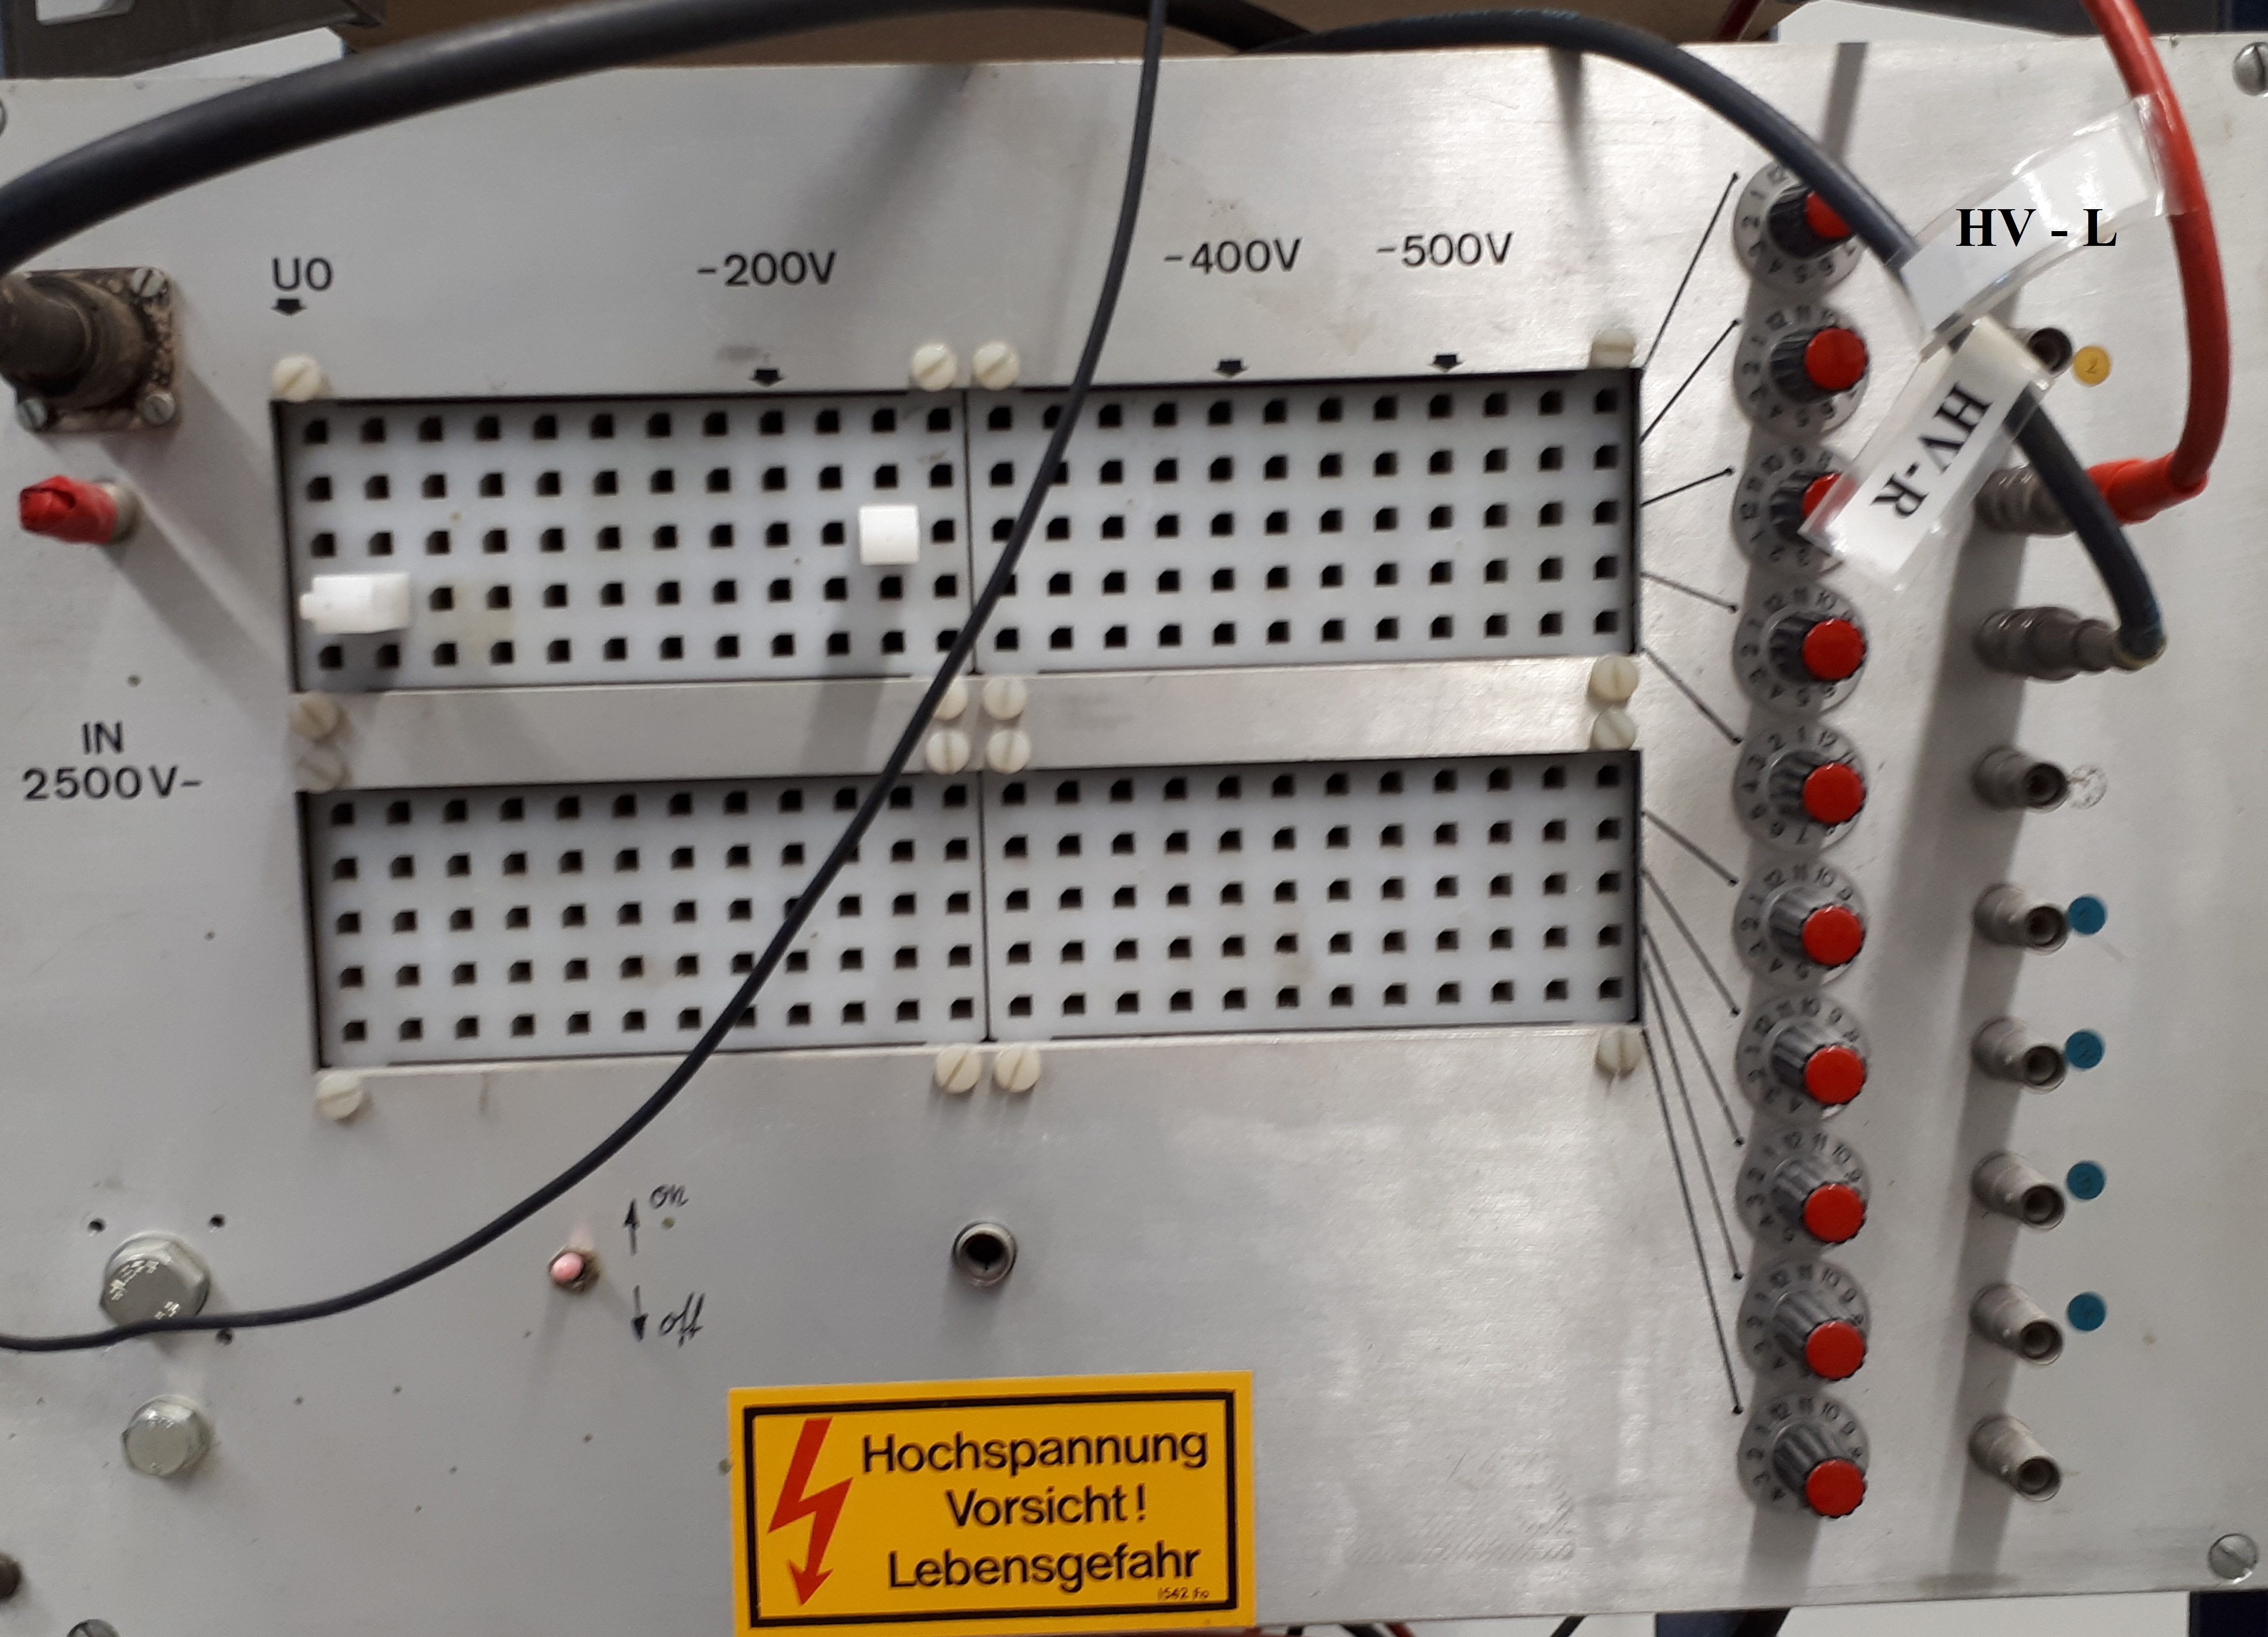
\includegraphics[width=\linewidth]{Plots/Spannung.jpg}
\caption{Picture of the voltage distribution for similar PMT signals. HV-L (red) supplies the left PMT and HV-R (black) the right one.}
\label{fig:voltage}
\end{subfigure}
\begin{subfigure}{0.45\textwidth}
\centering
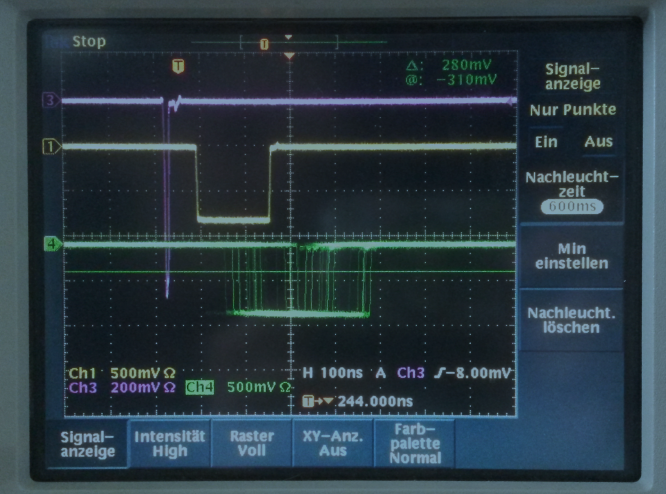
\includegraphics[width=\linewidth]{Plots/SignalOrder.png}
\caption{Picture of how the signals are received in the TDC. This displays the schemata shown in figure \ref{fig:timing}. Trigger, left PMT and at last right PMT. }
\label{fig:signal order}
\end{subfigure}
\caption{Set up and configuration. For detailed information see captions.}
\end{figure}

At the end of the configuration part we had to check if the order of delayed outputs and trigger signal from the gate generators DEL-output are correct. By triggering on the trigger signal we were able to reproduce the picture given in the script, see figure \ref{fig:signal order}. We forgot to take a picture by ourself but the trigger signal was on channel 1.


\subsection{Time calibration}\label{time}
For this chapter we placed a $^{207}Bi$ source on top of the scintillator. A folding yardstick was fasten on top. For the calibration we placed the source at $100cm$ which is the middle of the scintillator. This should result in equal time delay, if the Delay Boxes are not used and the same cables are used. To determine at which time unit the most events occurred each $50\ 000$ events were measured to create a histogram. This treatment stays the same for the following calibration and the determination of the speed of light c.

Because we have no value how many time units are equal to $1ns$, the calibration has to be done. We started with an offset of $32ns$ on the delay boxes, to ensure that the left PMT always starts the coincidence gate for the sake of consistency. By increasing the additional delay the time difference will rise too and therefore a proportionality will be visible.

Each data set of $50\ 000$ events is presented in the histograms in the Appendix \ref{appendix}. Each is fitted by the Gaussian function, where $\mu$ is the expected value, $\sigma$ the standard derivation, A the maximum amount at $\mu$ and b a constant off-set. 
\begin{equation}
n(x) = A\cdot exp \left( -\frac{(x-\mu)^2}{2\sigma^2} \right) + b
\end{equation}

We are especially interested in the expected value $\mu$. The slope of this time difference and the external delay will tell us the relation between the units of time given by the TDC and $1ns$. This comparison with a linear fit is shown in figure \ref{fig:TimeCalibration}.

\begin{figure}[H]
\centering
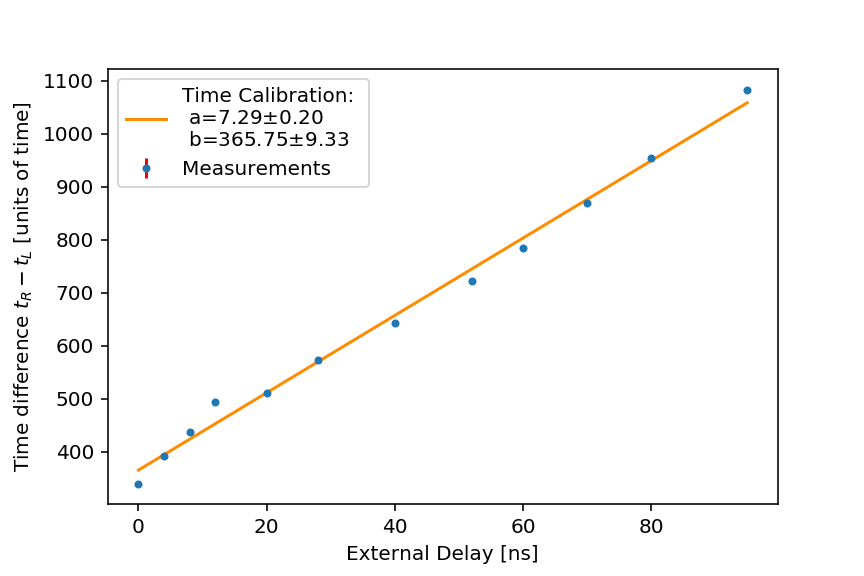
\includegraphics[width=1\textwidth]{Plots/TimeCalibration.png}
\caption{Expected values versus external delay. Identification of how many units of time are equal to one $1ns$. }
\label{fig:TimeCalibration}
\end{figure}

This concludes in in the following conversion rule, with the real time T [ns], time difference t [units of time] and slope $a$ as shown in figure \ref{fig:TimeCalibration}:
\begin{equation}
T = \frac{t}{a}\:,\: dT=\sqrt{\left(\frac{dt}{a}\right)^2 + \left(\frac{t\cdot da}{a^2}\right)^2}
\end{equation}

This large offset in the last mentioned figure is caused by the external delay to ensure a right order in signals. The zero delay is then equal to the constant delay for all measurements. It is about $32ns$ from the delay box plus the additional wire length. 
The shown errors are the uncertainty on the Gaussian fit parameters.


\subsection{Speed of light measurement}\label{c determination}
The same procedure is now applied to determine the speed of light in the plastic scintillator material. Instead of changing the delay of the right PMT it remains constant with $32ns$ plus additional cables. We took 41 sets of $50\ 000$ events, the individuals are shown in Appendix \ref{appendix}. For each measurement the position of the $^{207} Bi$ sample was changed by $4cm$. The error on the position is estimated with $0.5cm$, due to the size of the sample itself was around $0.8cm$. An example on how the individual sets of events are displayed is shown in figure \ref{fig:histogram20}.

\begin{figure}[H]
\centering
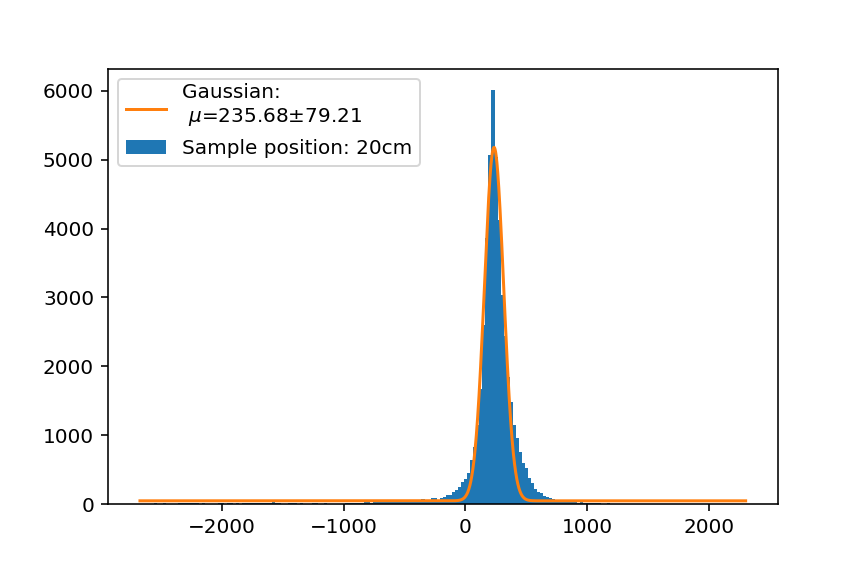
\includegraphics[width=1\textwidth]{Plots/Pos/20cm.png}
\caption{Histogram of events at the position of 20cm. }
\label{fig:histogram20}
\end{figure}

Again the expected values are plotted but now against the positions of the sample. The plots with units of time is shown in Appendix \ref{appendix} in figure \ref{fig:c fit units}. With the conversion rule at the end of chapter \ref{time}, the values for T are calculated. The results after linear regression are shown in figure \ref{fig:c fit}.

\begin{figure}[H]
\centering
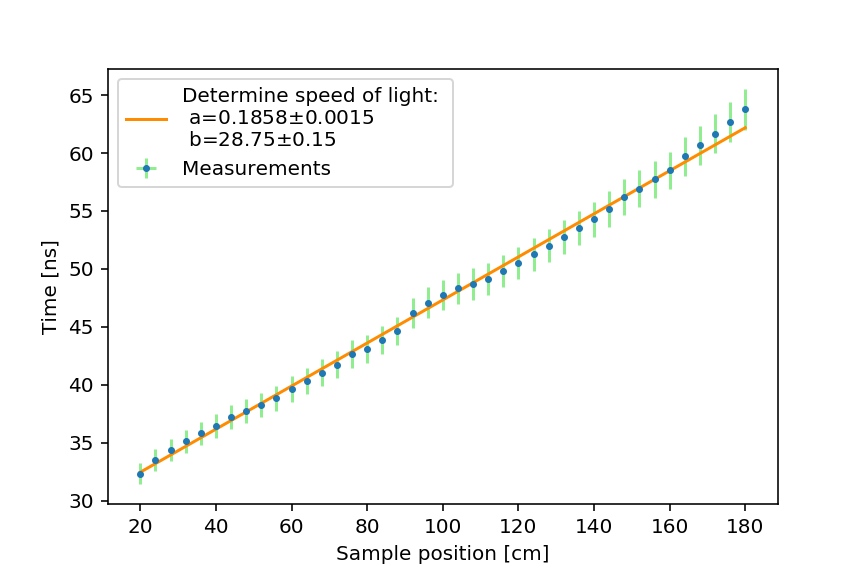
\includegraphics[width=1\textwidth]{Plots/PosTime.png}
\caption{Linear regression for the value of c. Converted time T against the samples position. }
\label{fig:c fit}
\end{figure}

Now by inverting the given slope we get our value for the speed of light in the plastic scintillator material. The error on this value will follow equation \ref{eq:c error}.
\begin{equation} \label{eq:c error}
c=\frac{1}{a'}\:,\: dc=\frac{da'}{a'^2}
\end{equation}

To reference our value we searched for the refractive index $n$ of plastic scintillator material, due to the equation $ c= c_0 / n$. This describes the speed of light in a material, where $c_0 = 299\ 792\ 458 \frac{m}{s}$ is the speed of light in vacuum. We found a value of $n=1.58$ \cite{refractive index} and the following comparison.

\begin{table}[H]
\centering
\begin{tabular}{c|c|c}
Value & Fraction $[c_0]$ & Real value [$\frac{m}{s}$] \\ \hline \hline
Literature & $0.633$ & $189\ 742\ 062$  \\ \hline
Measurement & $0.1796 \pm 0.1486$ & $ 53\ 830\ 777 \pm 445\ 371$ \\ \hline
\end{tabular}
\end{table}

The literature value is more than three times larger than our measured value. This is not explainable by some small errors in positioning or the fit functions. Either the time calibration is very bad or another effect occurs in this experiment, which has not been discussed yet.\\

In the scintillator the $\beta^- - $ and $\gamma -$ decay particles are inducing an electromagnetic shower. With bremsstrahlung and the photo electric effect the number of photons increases with every generation. Looking at one generation: Relative to the original incoming photon the resulting outgoing photons will have a relative angle. With this effect happening in the other two dimensions vertical to the path from source to PMT, the total length for the lights path is higher than expected. This assumption is comparable with the random walk model. If the real path is longer the photons are faster than expected. This could cause the large discrepancy to the literature value if the path is around three times larger. But a factor of three seems to much.


\section{Conclusion}
In the end our speed of light seems to be wrong. There is the possibility that a mistake occurred while calibrating the conversion rule. With a larger value for $a$ in chapter \ref{time} the determination of the speed of light fit $a'$ will be decreased, too. And this results in a higher value of c.

There should be no influence on the time difference caused by the signal transmission from MSCF-16 to the ADC and TDC, because the wires length was the same. A small error cause could be the shape of the signals the TDC is receiving. A delta function would be the best way to determine start and stop of this measurement. The output visualised was not as ideal as theoretical possible but seemed sufficient.

Maybe the chosen $32ns$ offset between right and left PMT signal was not enough. This could be the reason why the histograms are showing counts in the negative time difference. This also could affect the signal processing. In this case it is possible that fluctuations are able to affect the measurements.

%% vll fällt jonas noch was ein...  


\section{Appendix}\label{appendix}
\subsection{Time calibration}
\begin{figure}[H]
\centering
\medskip
\begin{subfigure}{0.48\textwidth}
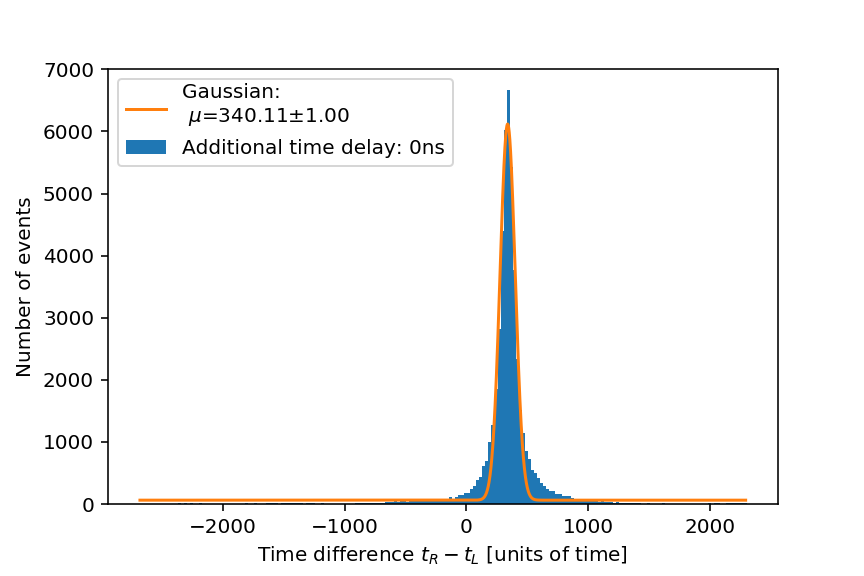
\includegraphics[width=\linewidth]{Plots/Time/0ns.png}
\end{subfigure}
\begin{subfigure}[c]{0.48\linewidth}
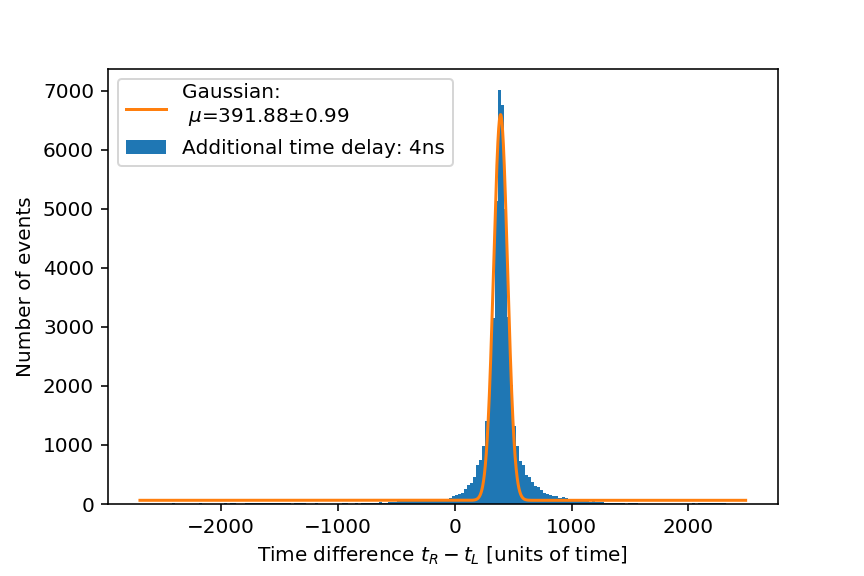
\includegraphics[width=\linewidth]{Plots/Time/4ns.png}
\end{subfigure}

\medskip
\begin{subfigure}{0.48\textwidth}
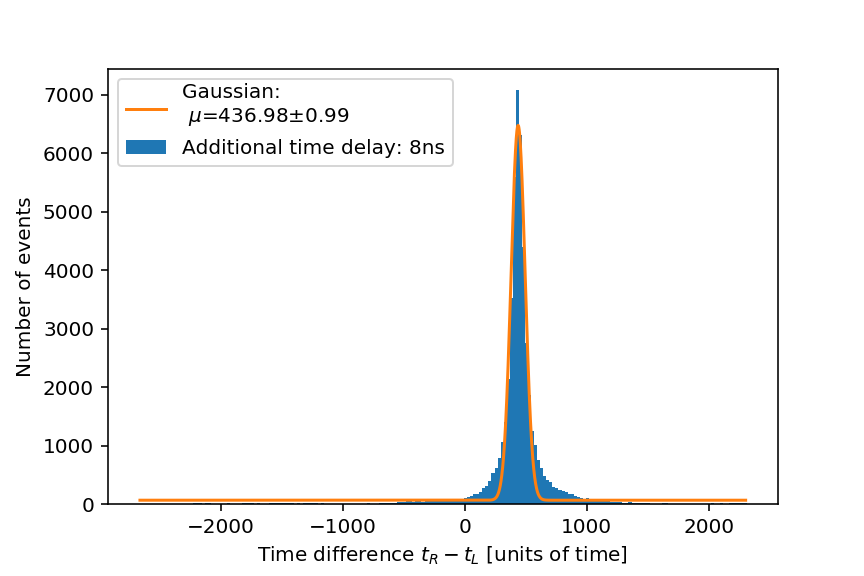
\includegraphics[width=\linewidth]{Plots/Time/8ns.png}
\end{subfigure}
\begin{subfigure}[c]{0.48\linewidth}
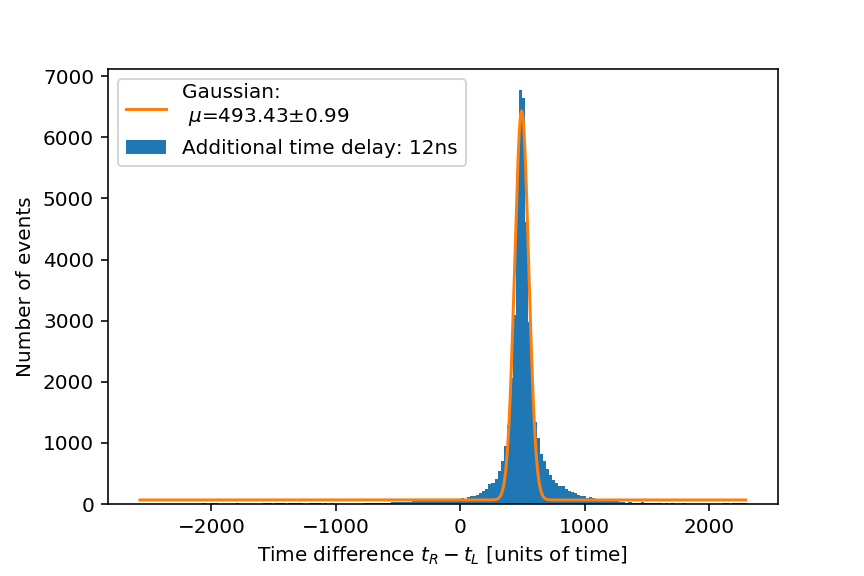
\includegraphics[width=\linewidth]{Plots/Time/12ns.png}
\end{subfigure}

\medskip
\begin{subfigure}{0.48\textwidth}
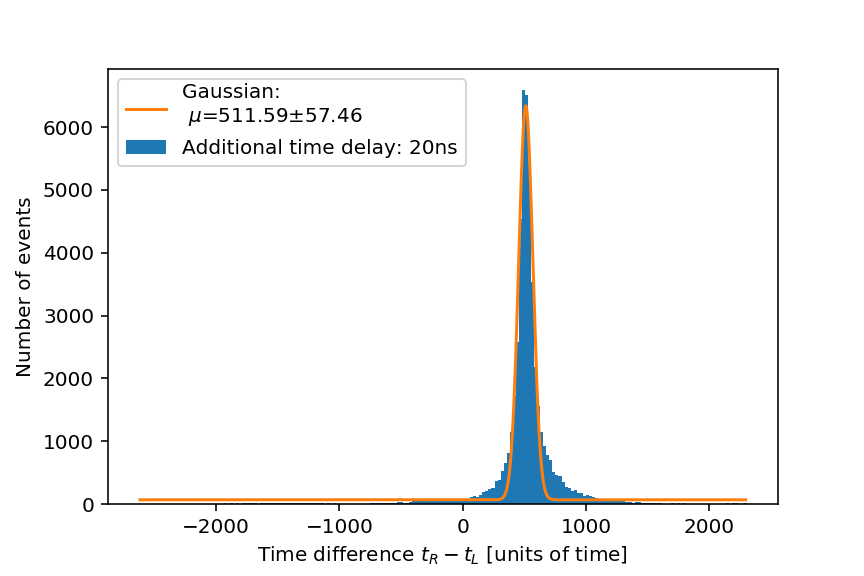
\includegraphics[width=\linewidth]{Plots/Time/20ns.png}
\end{subfigure}
\begin{subfigure}[c]{0.48\linewidth}
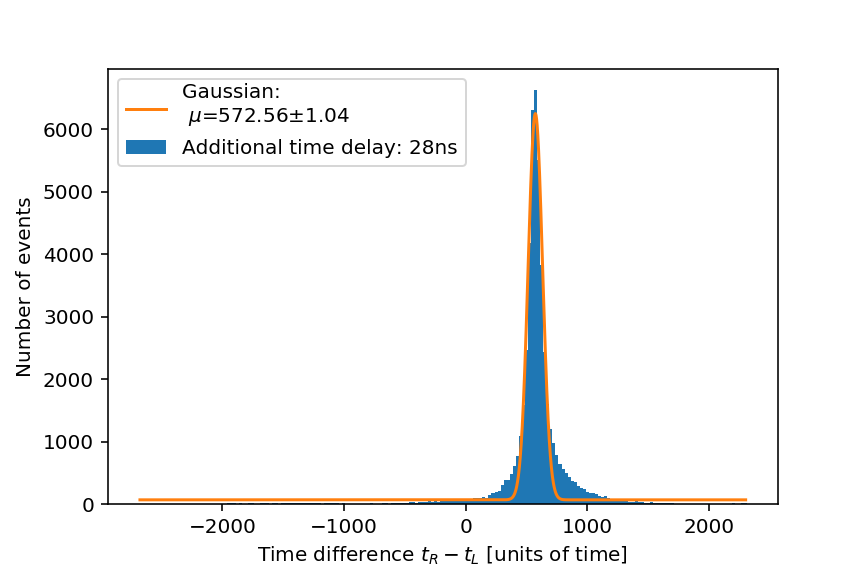
\includegraphics[width=\linewidth]{Plots/Time/28ns.png}
\end{subfigure}
\caption{Histograms for the time calibration in chapter \ref{time}. Part I }
\end{figure}

\begin{figure}[H]
\centering
\medskip
\begin{subfigure}{0.48\textwidth}
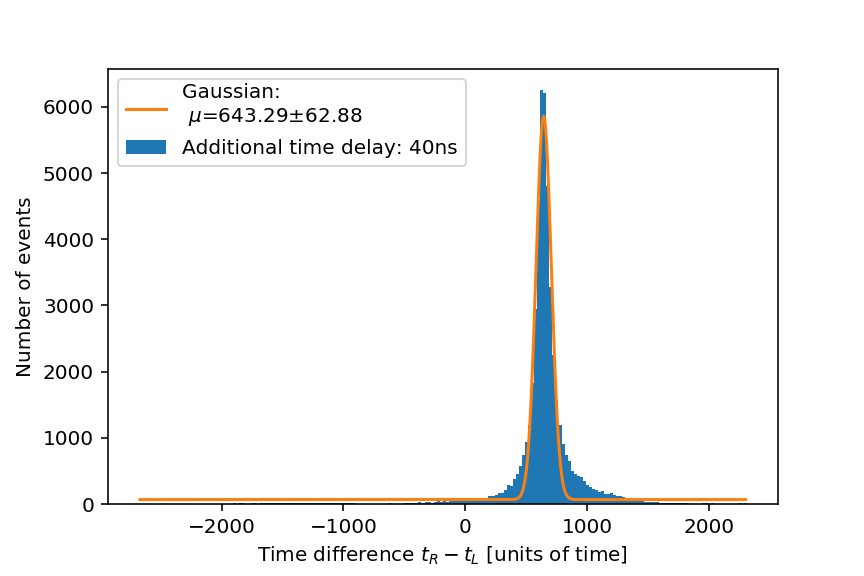
\includegraphics[width=\linewidth]{Plots/Time/40ns.png}
\end{subfigure}
\begin{subfigure}[c]{0.48\linewidth}
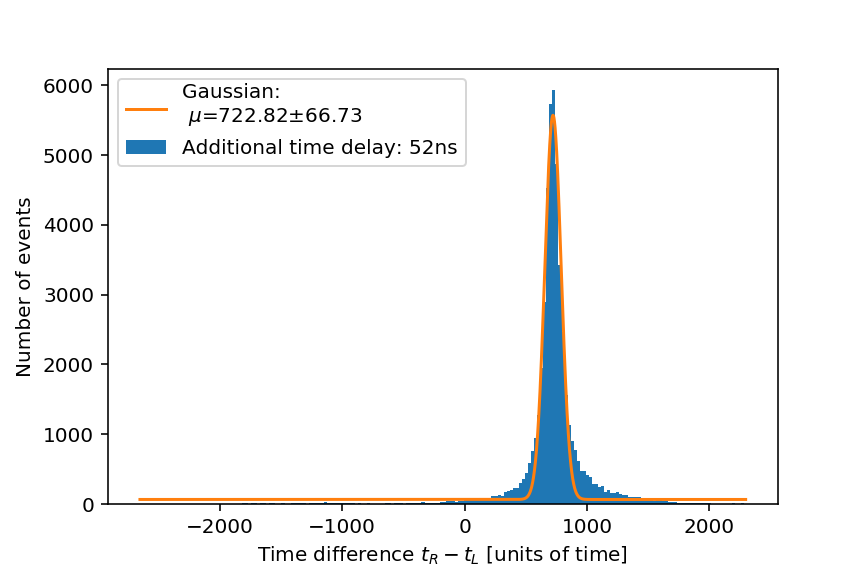
\includegraphics[width=\linewidth]{Plots/Time/52ns.png}
\end{subfigure}

\medskip
\begin{subfigure}{0.48\textwidth}
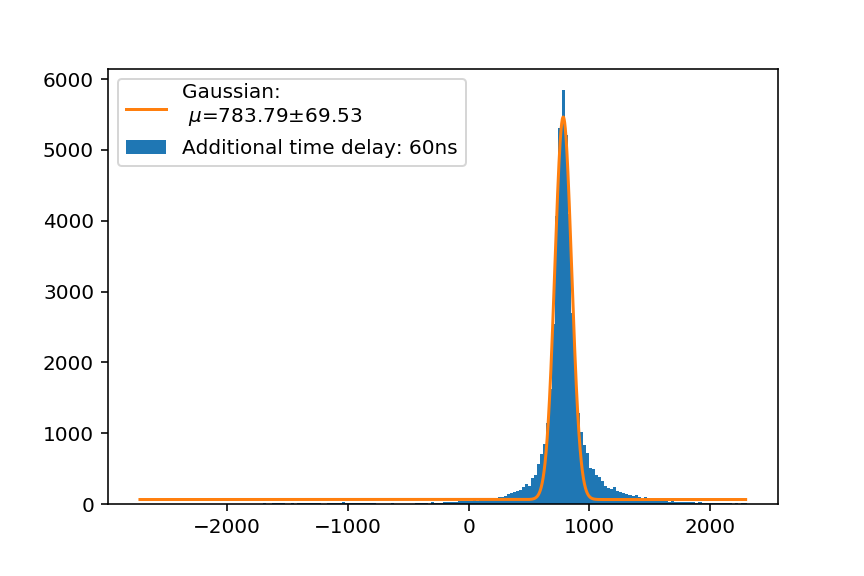
\includegraphics[width=\linewidth]{Plots/Time/60ns.png}
\end{subfigure}
\begin{subfigure}[c]{0.48\linewidth}
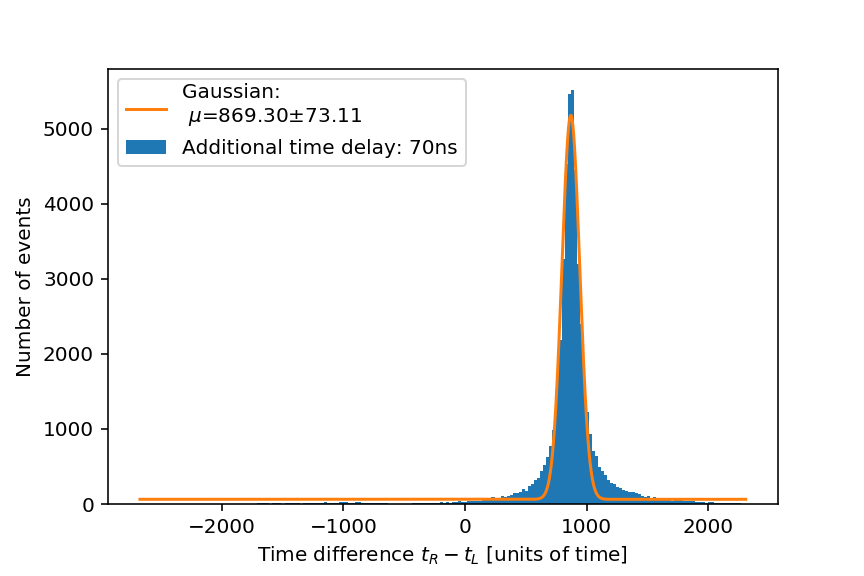
\includegraphics[width=\linewidth]{Plots/Time/70ns.png}
\end{subfigure}

\medskip
\begin{subfigure}{0.48\textwidth}
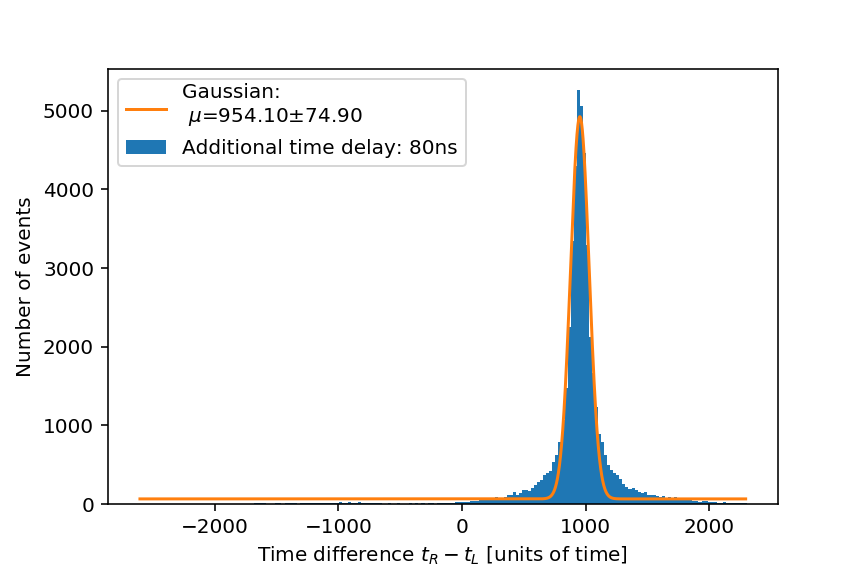
\includegraphics[width=\linewidth]{Plots/Time/80ns.png}
\end{subfigure}
\begin{subfigure}[c]{0.48\linewidth}
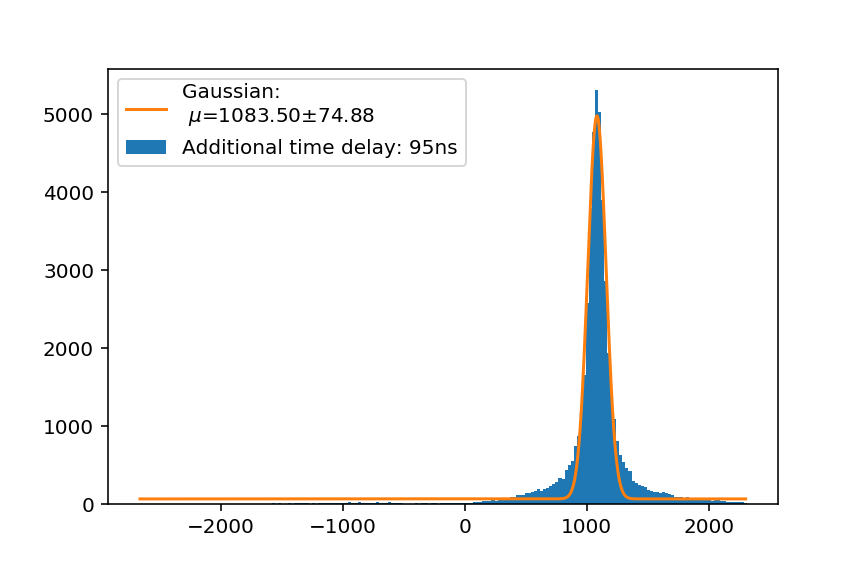
\includegraphics[width=\linewidth]{Plots/Time/95ns.png}
\end{subfigure}
\caption{Histograms for the time calibration in chapter \ref{time}. Part II }
\end{figure}


\subsection{Speed of light}
\begin{figure}[H]
\centering
\medskip
\begin{subfigure}{0.48\textwidth}
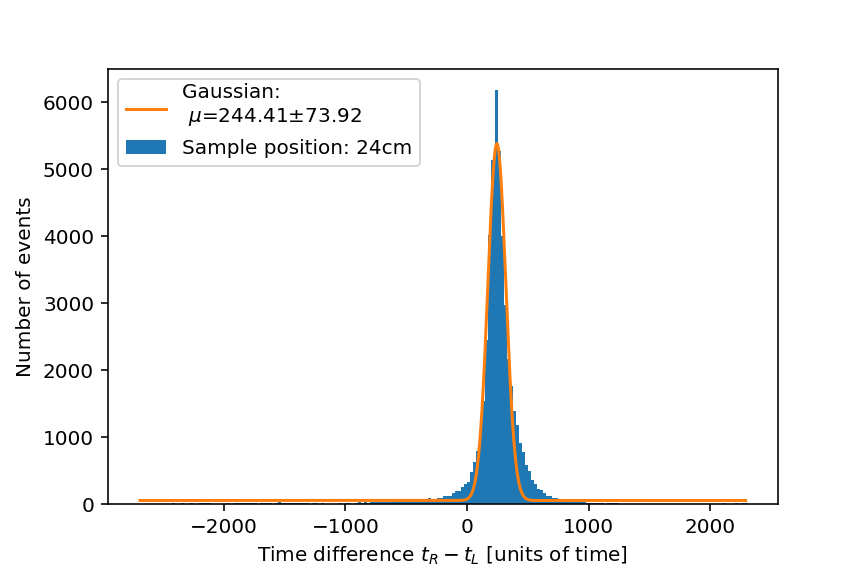
\includegraphics[width=\linewidth]{Plots/Pos/24cm.png}
\end{subfigure}
\begin{subfigure}[c]{0.48\linewidth}
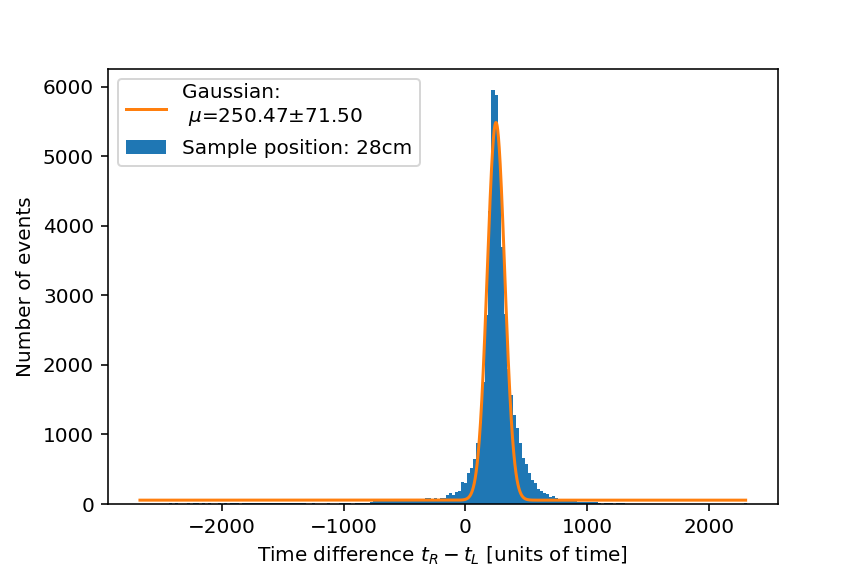
\includegraphics[width=\linewidth]{Plots/Pos/28cm.png}
\end{subfigure}

\medskip
\begin{subfigure}{0.48\textwidth}
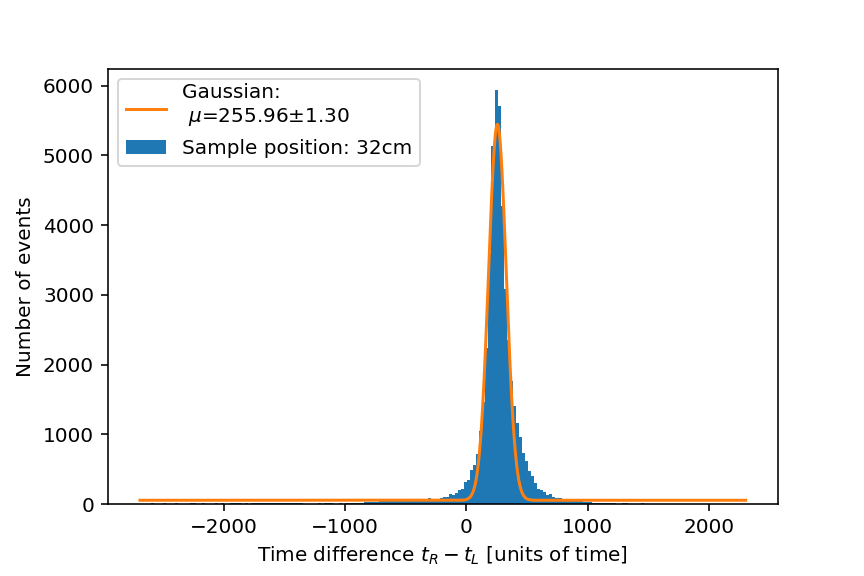
\includegraphics[width=\linewidth]{Plots/Pos/32cm.png}
\end{subfigure}
\begin{subfigure}[c]{0.48\linewidth}
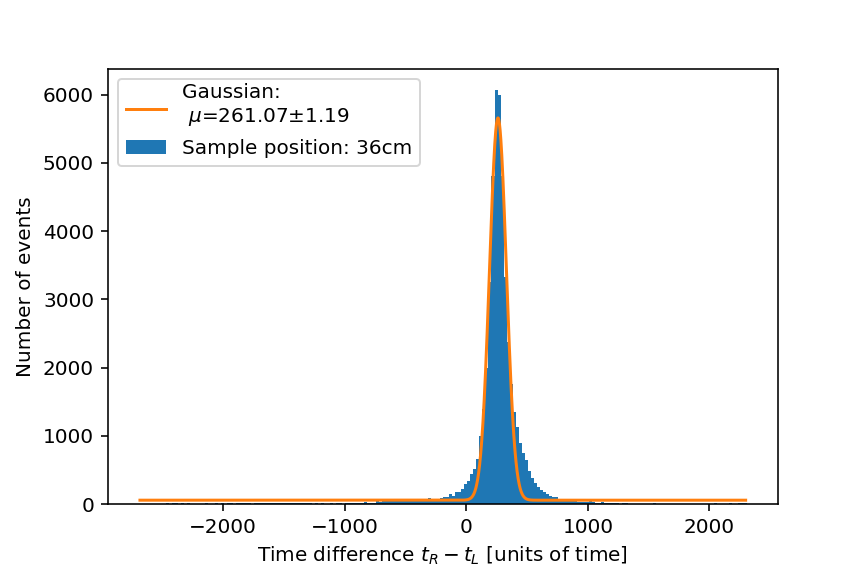
\includegraphics[width=\linewidth]{Plots/Pos/36cm.png}
\end{subfigure}

\medskip
\begin{subfigure}{0.48\textwidth}
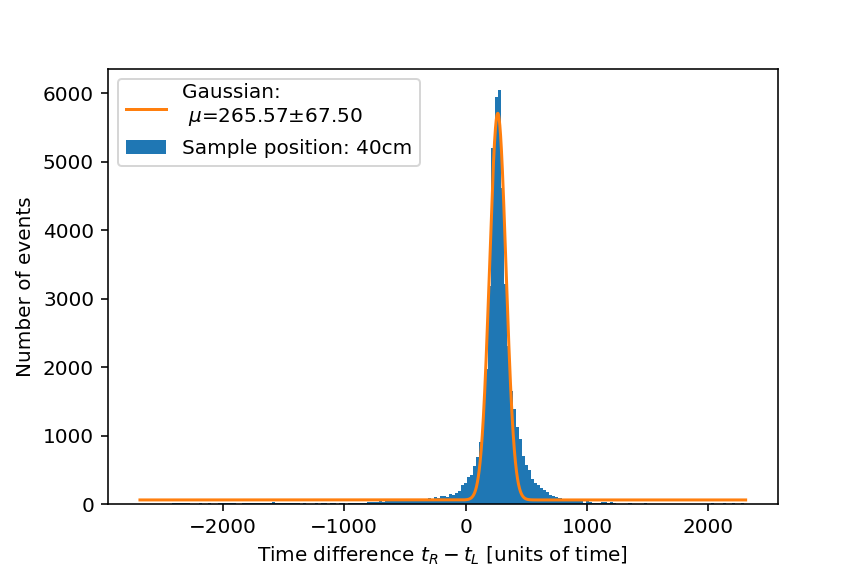
\includegraphics[width=\linewidth]{Plots/Pos/40cm.png}
\end{subfigure}
\begin{subfigure}[c]{0.48\linewidth}
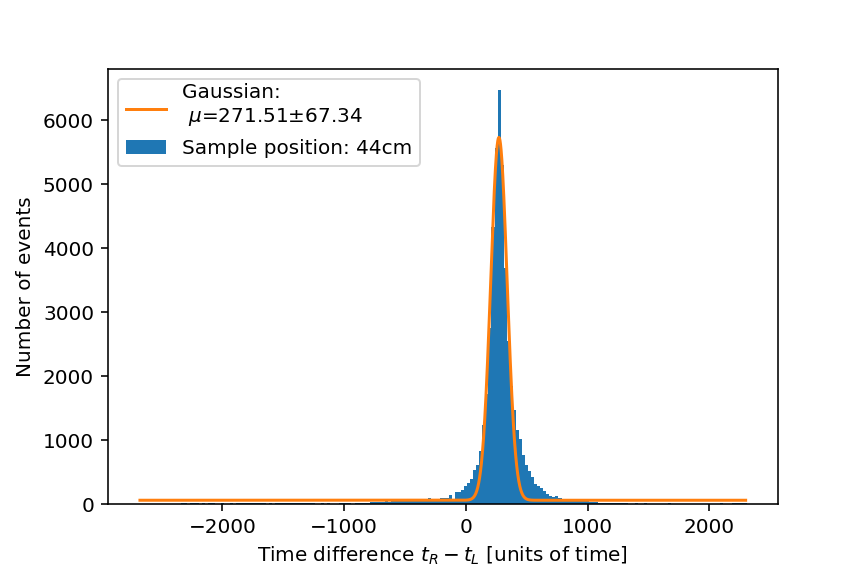
\includegraphics[width=\linewidth]{Plots/Pos/44cm.png}
\end{subfigure}

\medskip
\begin{subfigure}{0.48\textwidth}
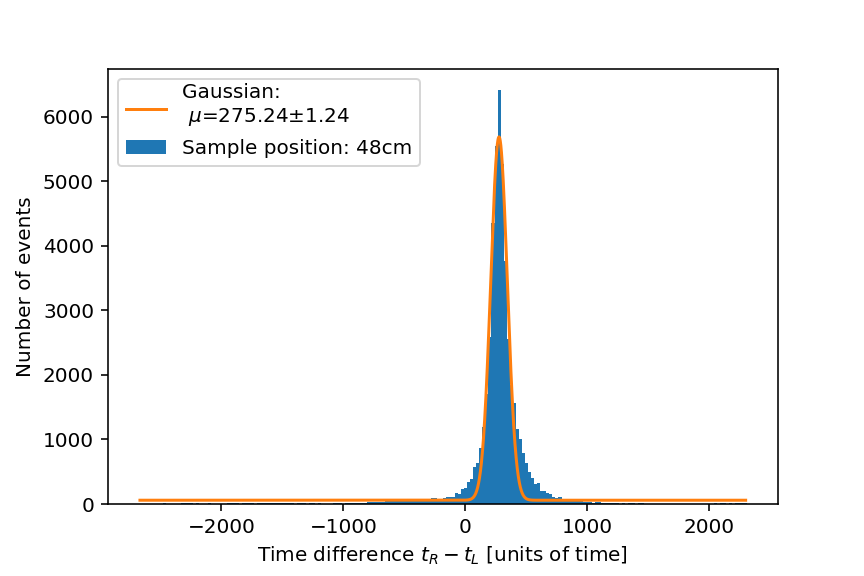
\includegraphics[width=\linewidth]{Plots/Pos/48cm.png}
\end{subfigure}
\begin{subfigure}[c]{0.48\linewidth}
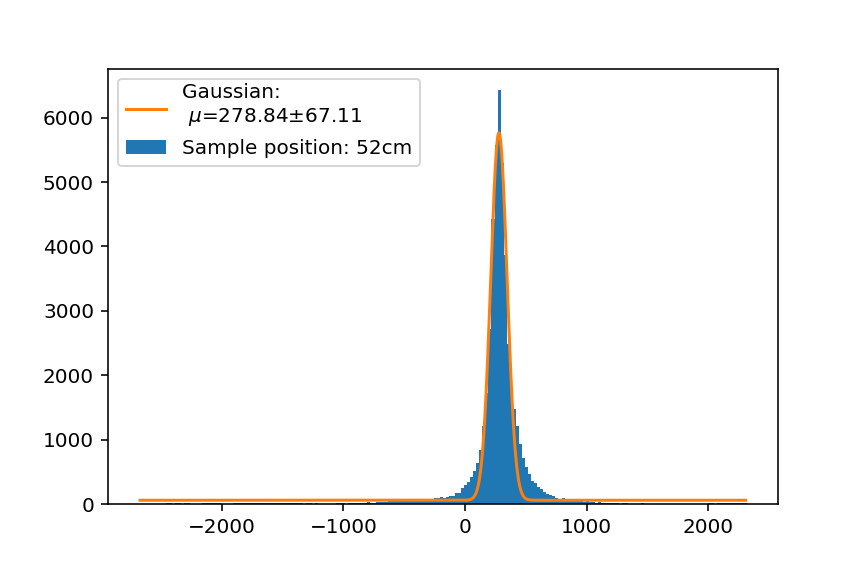
\includegraphics[width=\linewidth]{Plots/Pos/52cm.png}
\end{subfigure}
\caption{Histograms for the c calculation in chapter \ref{c determination}. Part I }
\end{figure}

\begin{figure}[H]
\centering
\medskip
\begin{subfigure}{0.48\textwidth}
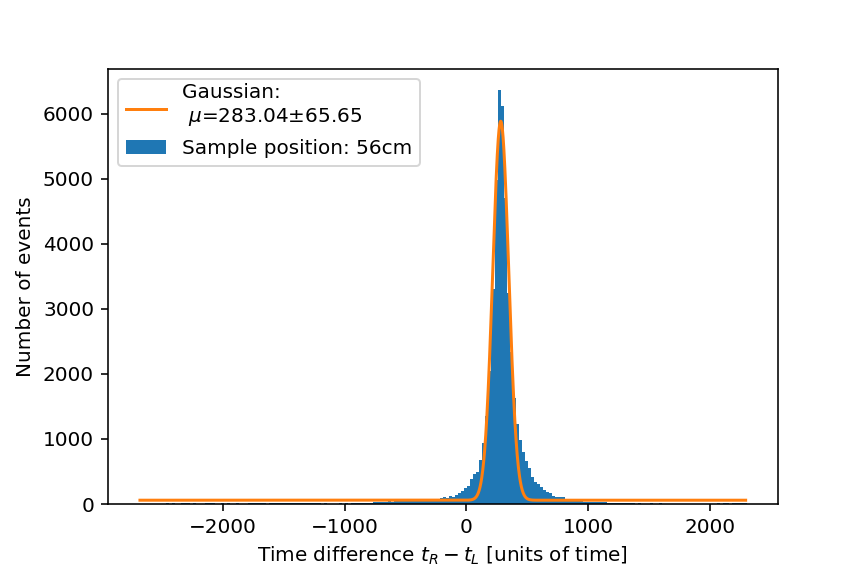
\includegraphics[width=\linewidth]{Plots/Pos/56cm.png}
\end{subfigure}
\begin{subfigure}[c]{0.48\linewidth}
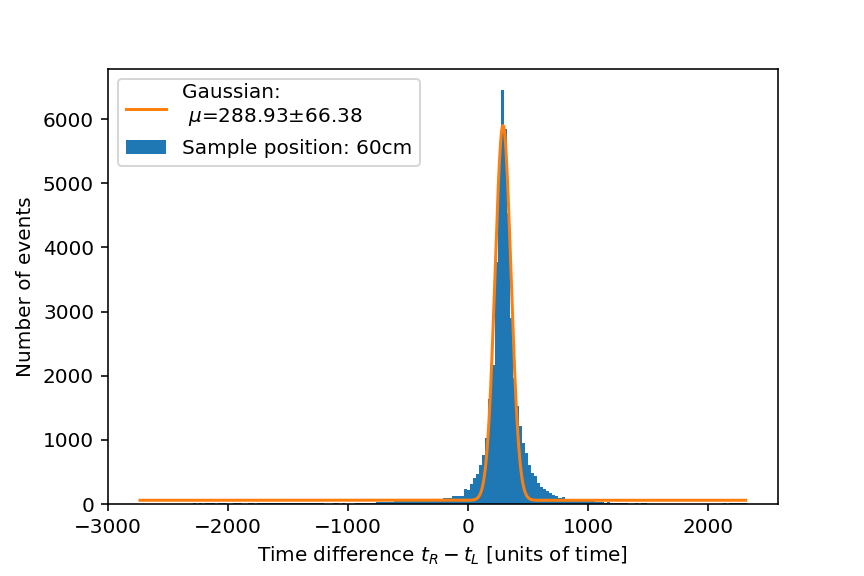
\includegraphics[width=\linewidth]{Plots/Pos/60cm.png}
\end{subfigure}

\medskip
\begin{subfigure}{0.48\textwidth}
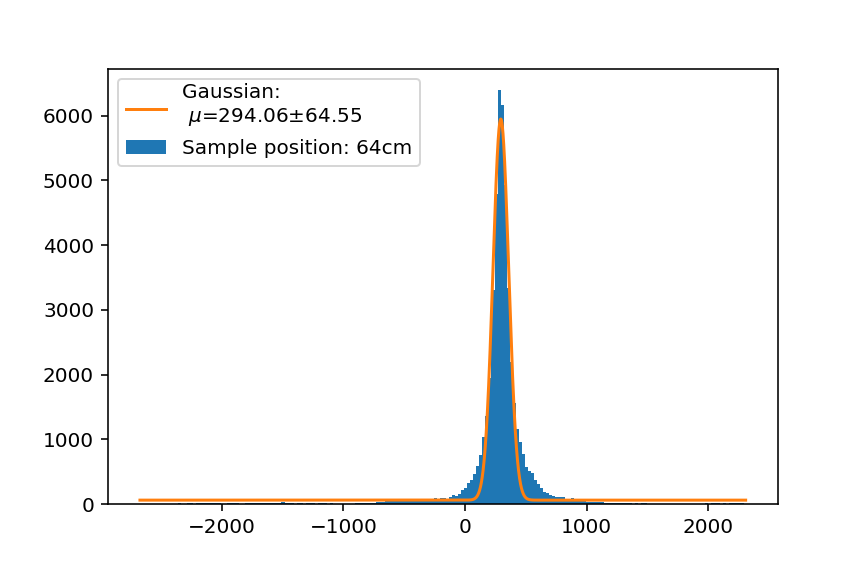
\includegraphics[width=\linewidth]{Plots/Pos/64cm.png}
\end{subfigure}
\begin{subfigure}[c]{0.48\linewidth}
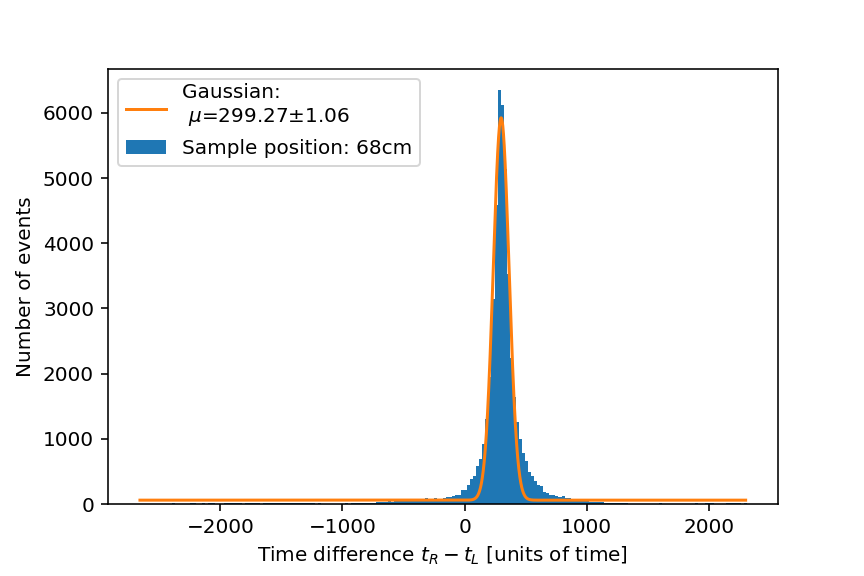
\includegraphics[width=\linewidth]{Plots/Pos/68cm.png}
\end{subfigure}

\medskip
\begin{subfigure}{0.48\textwidth}
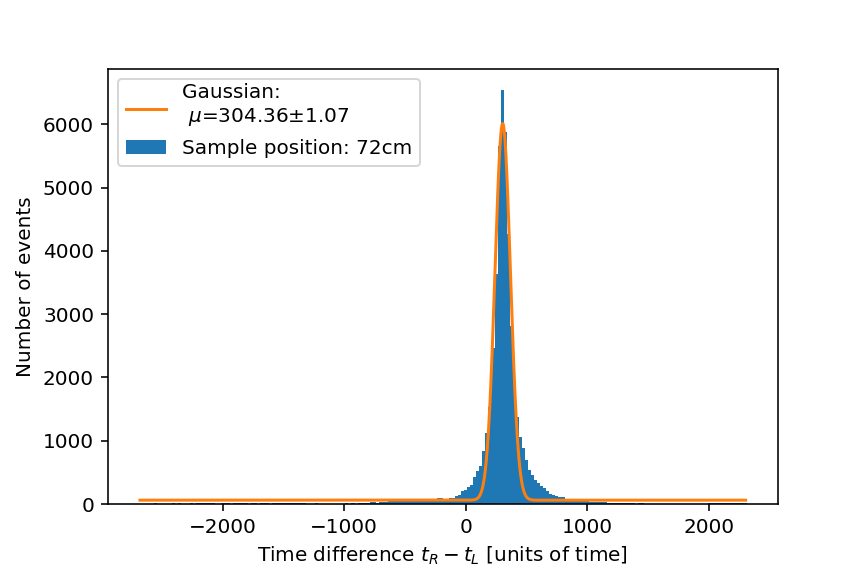
\includegraphics[width=\linewidth]{Plots/Pos/72cm.png}
\end{subfigure}
\begin{subfigure}[c]{0.48\linewidth}
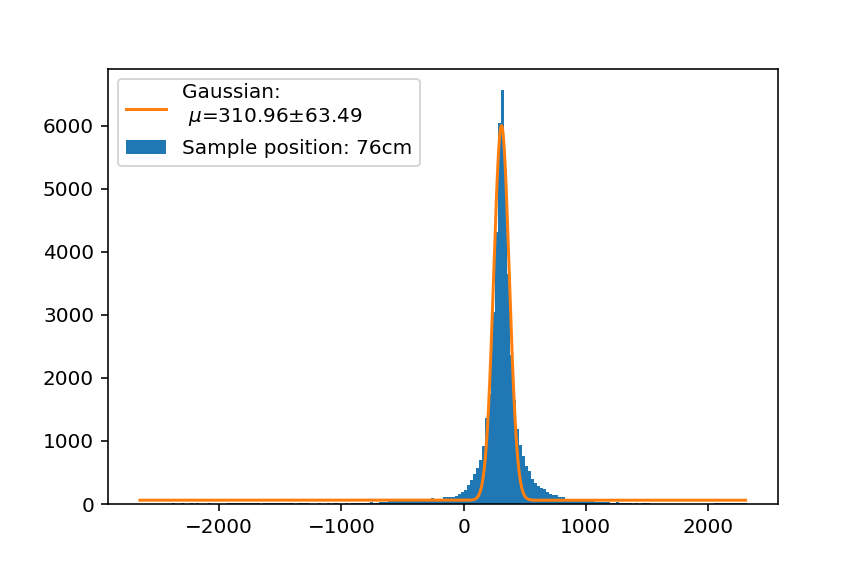
\includegraphics[width=\linewidth]{Plots/Pos/76cm.png}
\end{subfigure}

\medskip
\begin{subfigure}{0.48\textwidth}
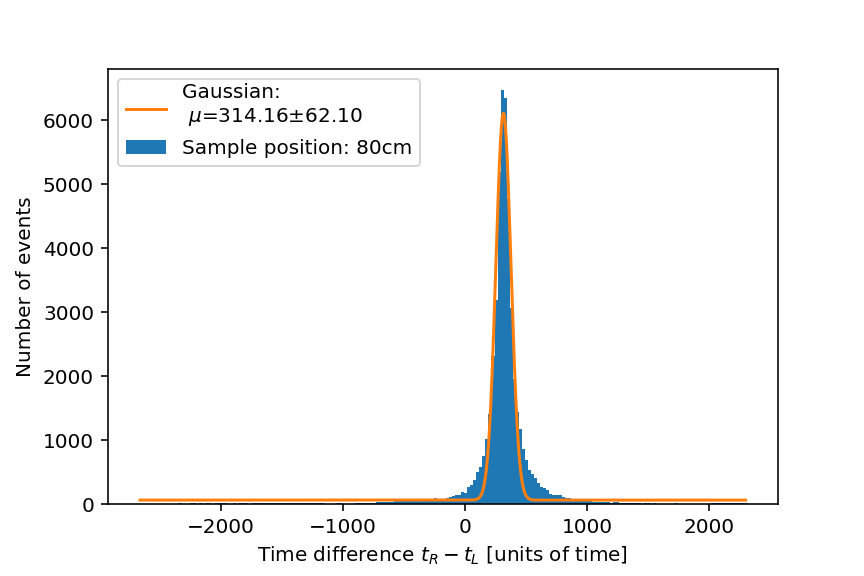
\includegraphics[width=\linewidth]{Plots/Pos/80cm.png}
\end{subfigure}
\begin{subfigure}[c]{0.48\linewidth}
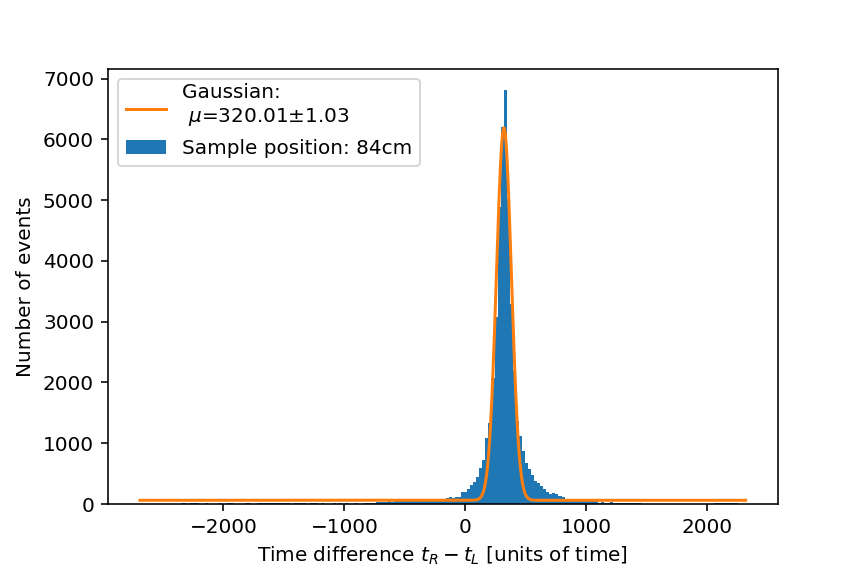
\includegraphics[width=\linewidth]{Plots/Pos/84cm.png}
\end{subfigure}
\caption{Histograms for the c calculation in chapter \ref{c determination}. Part II }
\end{figure}

\begin{figure}[H]
\centering
\medskip
\begin{subfigure}{0.48\textwidth}
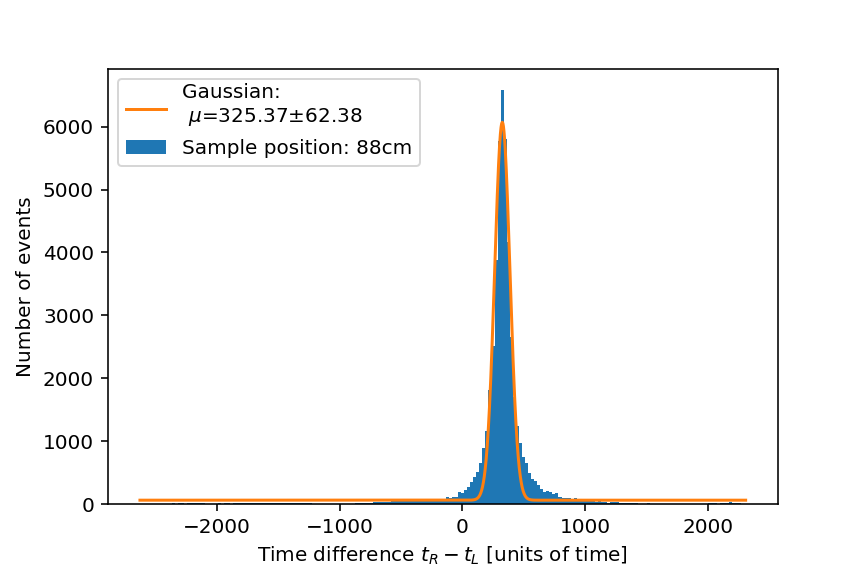
\includegraphics[width=\linewidth]{Plots/Pos/88cm.png}
\end{subfigure}
\begin{subfigure}[c]{0.48\linewidth}
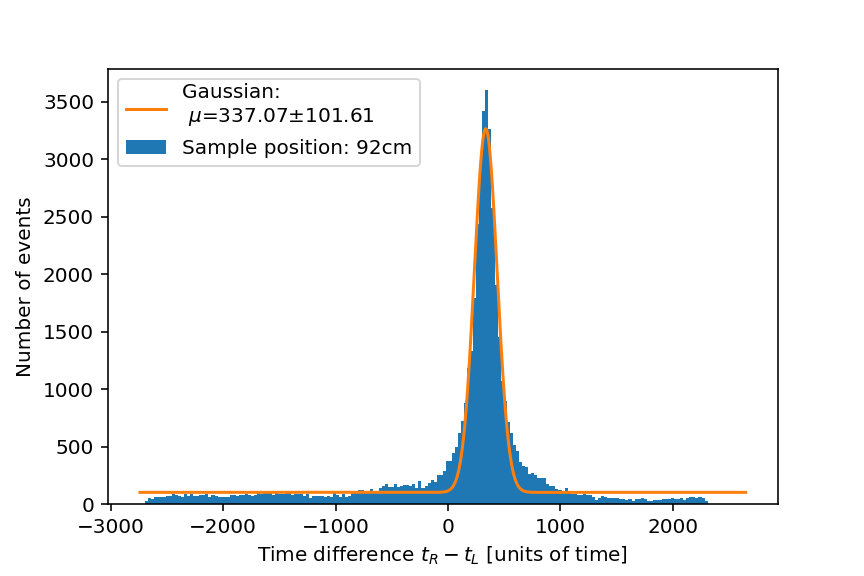
\includegraphics[width=\linewidth]{Plots/Pos/92cm.png}
\end{subfigure}

\medskip
\begin{subfigure}{0.48\textwidth}
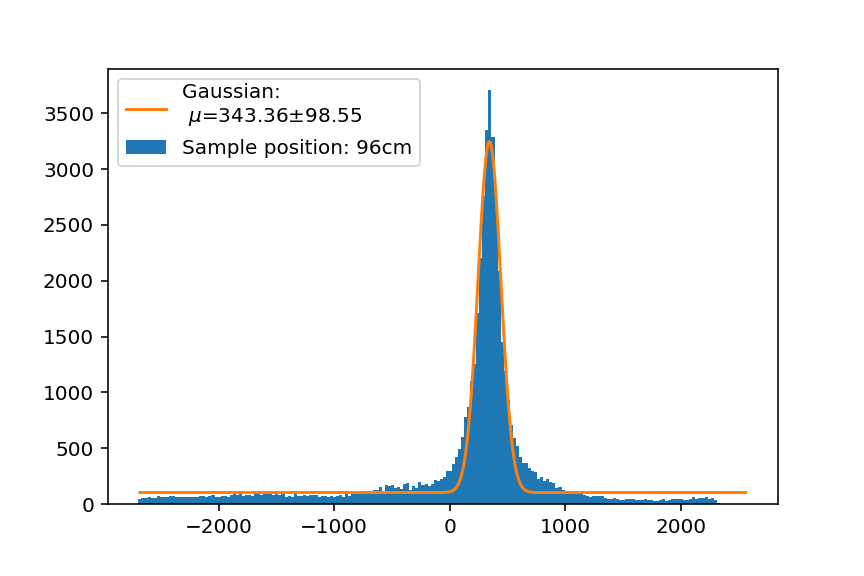
\includegraphics[width=\linewidth]{Plots/Pos/96cm.png}
\end{subfigure}
\begin{subfigure}[c]{0.48\linewidth}
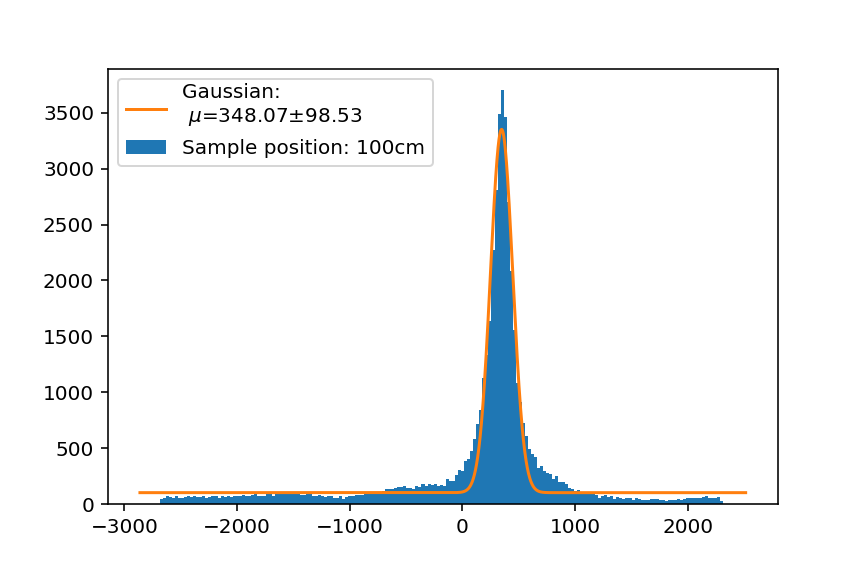
\includegraphics[width=\linewidth]{Plots/Pos/100cm.png}
\end{subfigure}

\medskip
\begin{subfigure}{0.48\textwidth}
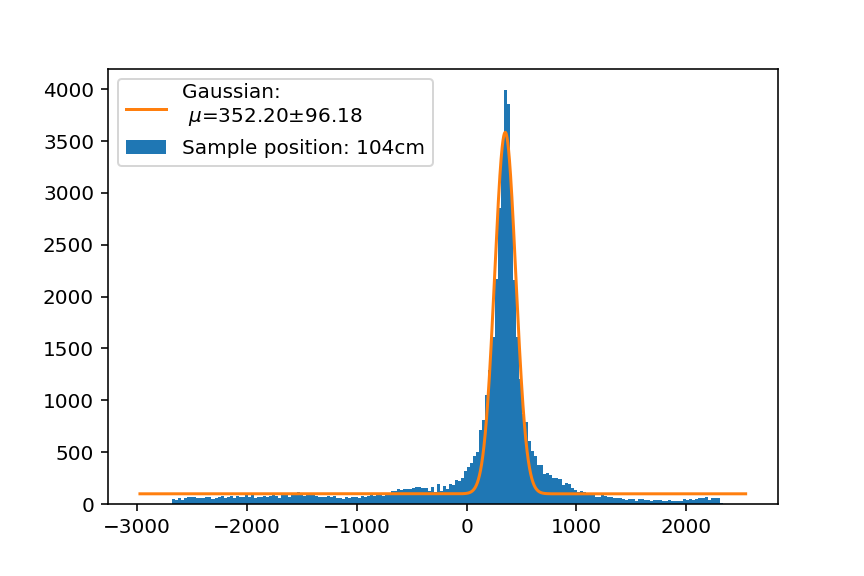
\includegraphics[width=\linewidth]{Plots/Pos/104cm.png}
\end{subfigure}
\begin{subfigure}[c]{0.48\linewidth}
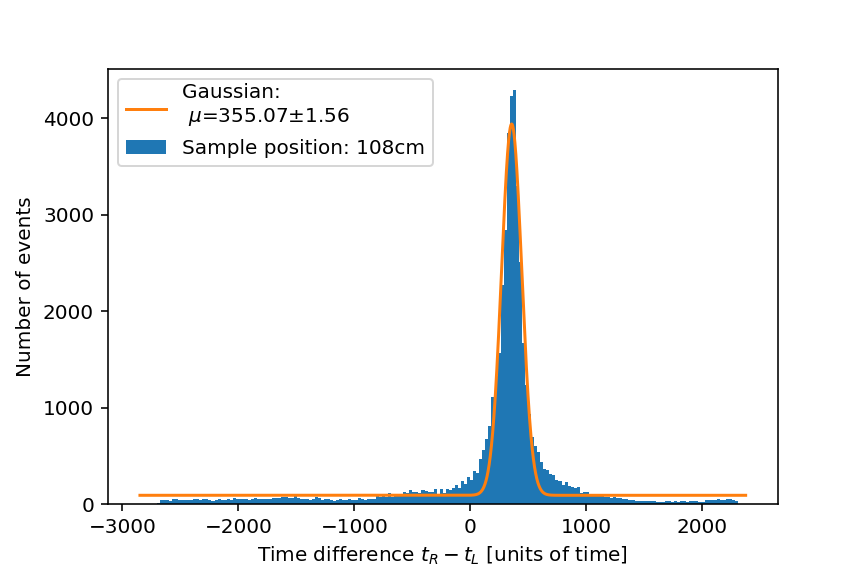
\includegraphics[width=\linewidth]{Plots/Pos/108cm.png}
\end{subfigure}

\medskip
\begin{subfigure}{0.48\textwidth}
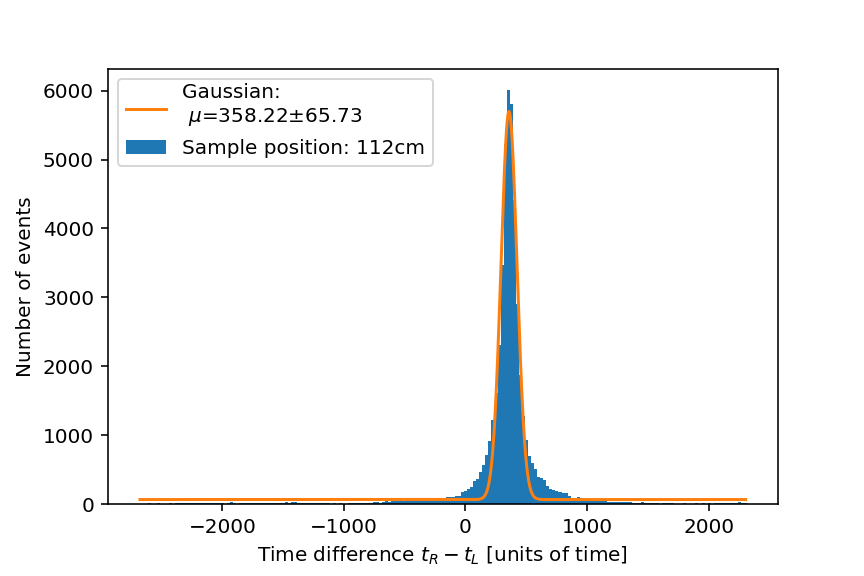
\includegraphics[width=\linewidth]{Plots/Pos/112cm.png}
\end{subfigure}
\begin{subfigure}[c]{0.48\linewidth}
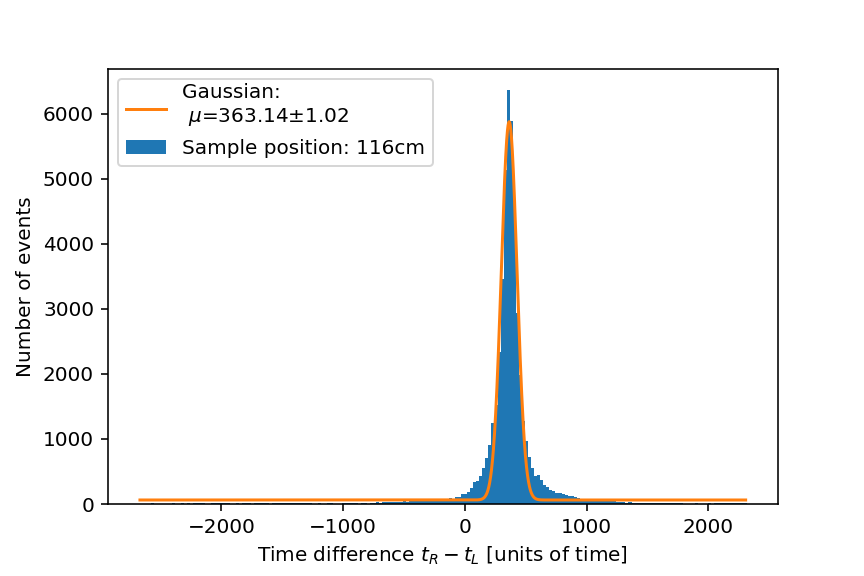
\includegraphics[width=\linewidth]{Plots/Pos/116cm.png}
\end{subfigure}
\caption{Histograms for the c calculation in chapter \ref{c determination}. Part III }
\end{figure}

\begin{figure}[H]
\centering
\medskip
\begin{subfigure}{0.48\textwidth}
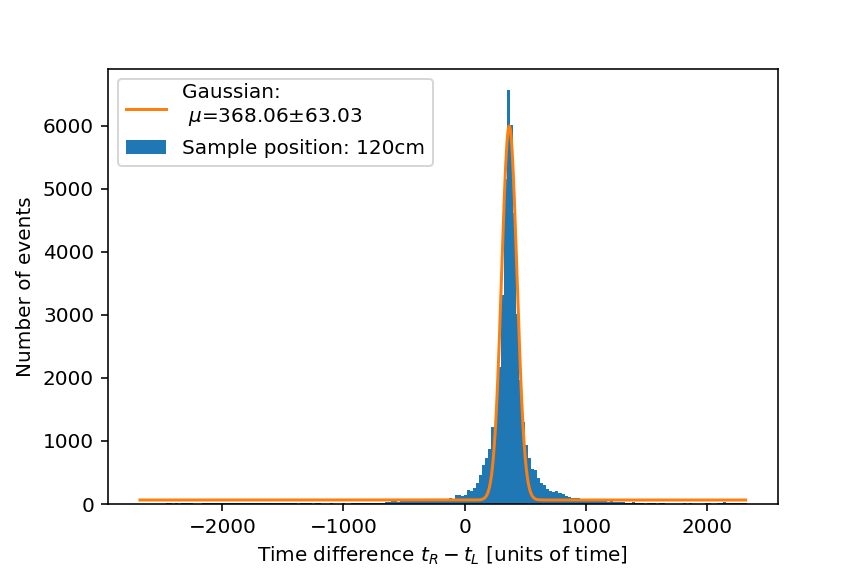
\includegraphics[width=\linewidth]{Plots/Pos/120cm.png}
\end{subfigure}
\begin{subfigure}[c]{0.48\linewidth}
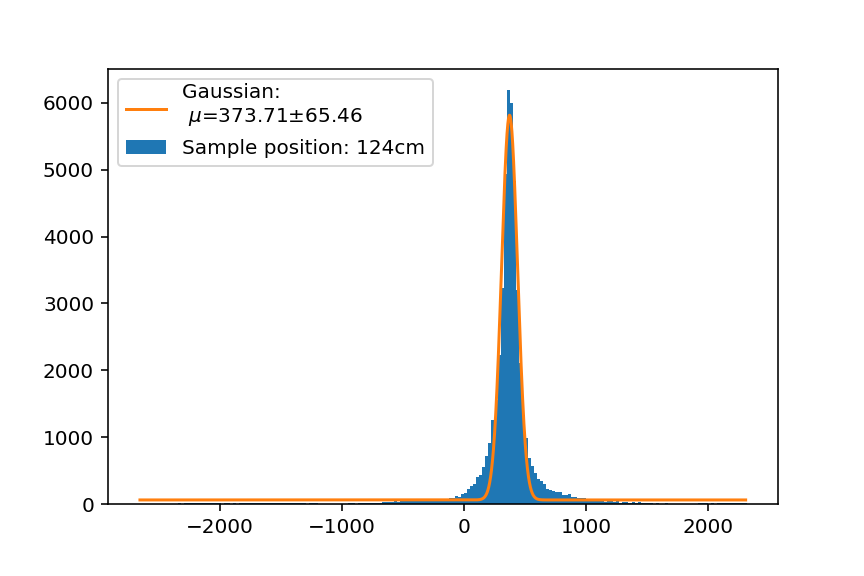
\includegraphics[width=\linewidth]{Plots/Pos/124cm.png}
\end{subfigure}

\medskip
\begin{subfigure}{0.48\textwidth}
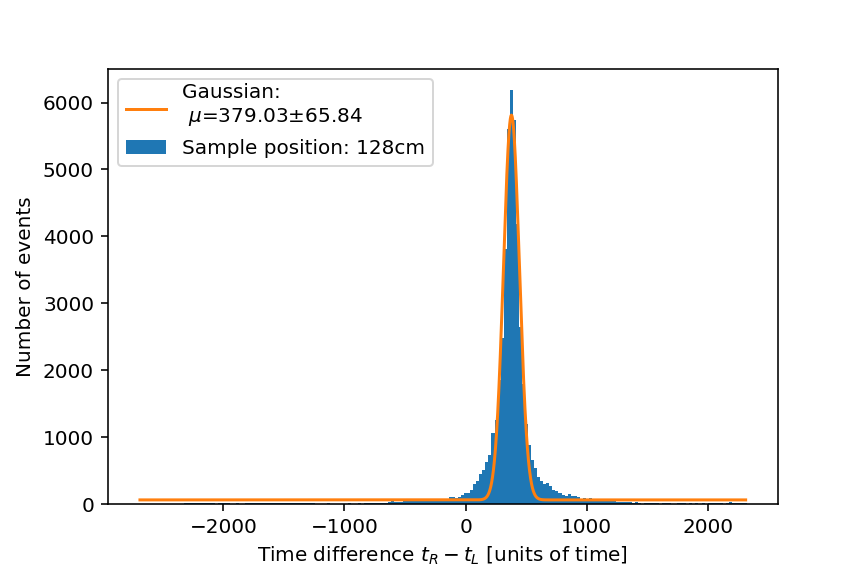
\includegraphics[width=\linewidth]{Plots/Pos/128cm.png}
\end{subfigure}
\begin{subfigure}[c]{0.48\linewidth}
\includegraphics[width=\linewidth]{Plots/Pos/132cm.png}
\end{subfigure}

\medskip
\begin{subfigure}{0.48\textwidth}
\includegraphics[width=\linewidth]{Plots/Pos/136cm.png}
\end{subfigure}
\begin{subfigure}[c]{0.48\linewidth}
\includegraphics[width=\linewidth]{Plots/Pos/140cm.png}
\end{subfigure}

\medskip
\begin{subfigure}{0.48\textwidth}
\includegraphics[width=\linewidth]{Plots/Pos/144cm.png}
\end{subfigure}
\begin{subfigure}[c]{0.48\linewidth}
\includegraphics[width=\linewidth]{Plots/Pos/148cm.png}
\end{subfigure}
\caption{Histograms for the time calibration in chapter \ref{time}. Part IV }
\end{figure}

\begin{figure}[H]
\centering
\medskip
\begin{subfigure}{0.48\textwidth}
\includegraphics[width=\linewidth]{Plots/Pos/152cm.png}
\end{subfigure}
\begin{subfigure}[c]{0.48\linewidth}
\includegraphics[width=\linewidth]{Plots/Pos/156cm.png}
\end{subfigure}

\medskip
\begin{subfigure}{0.48\textwidth}
\includegraphics[width=\linewidth]{Plots/Pos/160cm.png}
\end{subfigure}
\begin{subfigure}[c]{0.48\linewidth}
\includegraphics[width=\linewidth]{Plots/Pos/164cm.png}
\end{subfigure}

\medskip
\begin{subfigure}{0.48\textwidth}
\includegraphics[width=\linewidth]{Plots/Pos/168cm.png}
\end{subfigure}
\begin{subfigure}[c]{0.48\linewidth}
\includegraphics[width=\linewidth]{Plots/Pos/172cm.png}
\end{subfigure}

\medskip
\begin{subfigure}{0.48\textwidth}
\includegraphics[width=\linewidth]{Plots/Pos/176cm.png}
\end{subfigure}
\begin{subfigure}[c]{0.48\linewidth}
\includegraphics[width=\linewidth]{Plots/Pos/180cm.png}
\end{subfigure}
\caption{Histograms for the c calculation in chapter \ref{c determination}. Part V }
\end{figure}

\begin{figure}[H]
\centering
\includegraphics[width=1\textwidth]{Plots/PosTimeUnit.png}
\caption{Linear regression for the value of c. Original time units from the TDC against the samples position. }
\label{fig:c fit units}
\end{figure}

\newpage
\begin{thebibliography}{}

\bibitem{script} VMEScript.pdf, script for this experiment.

\bibitem{refractive index} \begin{verbatim}
https://eljentechnology.com/images/products/data_sheets/
  EJ-228_EJ-230.pdf
 https://www.crystals.saint-gobain.com/sites/imdf.crystals.com/
  files/documents/sgc-bc400-404-408-412-416-data-sheet.pdf
\end{verbatim} 

\bibitem{muon} \begin{verbatim}
http://cosmic.lbl.gov/SKliewer/Cosmic_Rays/Muons.htm
\end{verbatim}

\end{thebibliography}
\end{document}

